\section[Background]{Background\footnote{Sylvi Kuperman greatly assisted us in preparing this section of the appendix.}} \label{appendix:background}

\subsection{Overview}

\noindent The Carolina Abecedarian Project (ABC) and the Carolina Approach to Responsive Education (CARE) were high-quality early childhood education programs each with two phases of randomized controlled design. They were both implemented at the Frank Porter Graham Center (FPGC) of the University of North Carolina in Chapel Hill. ABC served four cohorts of children born between 1972 and 1977, and CARE served two cohorts of children born between 1977 and 1980. In this section of the appendix, we expand on important details of the eligibility requirements, the randomization protocol, and the programmatic contents of both programs.

\subsection{Eligibility Criteria and Populations Served}\label{app:eligibility-pop}

\noindent The mothers of the ABC and CARE subjects were generally recruited during the last trimester  of pregnancy. Potential families were referred by local social service agencies and hospitals. Eligibility was determined by a score of 11 or more on a weighted 13-factor High-risk Index (HRI). Table~\ref{table:hri-abc} details the items of the HRI for ABC.\\

\begin{table}[htbp]
\centering
\caption{High-risk Index for ABC}\label{table:hri-abc}
\scriptsize
\begin{tabular}{c L{30em} c c}
\toprule
& Item & Response & Weight \\
\midrule
1 	& Maternal education (years of education) & 6 & 8 \\
	& 								& 7 & 7 \\
	& 								& 8 & 6 \\
	&								& 9 & 3 \\
	&								& 10 & 2 \\
	&								& 11 & 1 \\
	& 								& 12 & 0 \\
2	& Paternal education (years of education) & \mc{2}{c}{same as maternal education} \\
3 	& Year family income (2014 USD) 	& \$5,663.54 or less & 8 \\
	&								& \$5,663.54-\$11,327.08 & 7 \\
	&								& \$11,327.08-\$16,990.62 & 6 \\
	&								& \$16,990.62-\$22,654.16 & 5 \\
	&								& \$22,654.16-\$28,317.70 & 4 \\
	&								& \$28,317.70-\$33,981.24 & 0 \\
4	& Father's absence from the household for reason other than health or death & Yes & 3 \\
5	& Lack of maternal relatives in the area	& Yes & 3 \\
6 	& Siblings in school age one or more	 grades behind age-appropriate level	 or low scores on school-administered achievement tests & Yes & 3 \\
7 	& Received payments from welfare agencies within the past 3 years	& Yes & 3 \\
8 	& Father's work unstable or unskilled and semi-skilled labor & Yes & 3 \\
9 	& Maternal or paternal IQ 90 or below	& Yes & 3 \\
10 	& Sibling with an IQ score 90 or below	& Yes & 3 \\
11	& Relevant social agencies indicate that family is in need of assistance & Yes & 3 \\
12 	& One or more family members has sought professional help in the past 3 years & Yes & 1 \\
13	& Special circumstances not included in any of the above that are likely contributors	to cultural or social disadvantage & Yes & 1 \\
\bottomrule
\end{tabular}
\justify
Note: This table shows the High-risk Index (HRI) for ABC. A score of 11 or more determined eligibility \citep{Ramey_Smith_1977_AJMD, Ramey_Campbell_1984_AJMD,Ramey_Campbell_1991_childreninpoverty,Ramey_Campbell_etal_2000_ADS}. The weighting scale aimed to establish the relative importance of each item in the index \citep{Ramey_Smith_1977_AJMD}. Race was not  considered for eligibility; however, 98\% of the families who agreed to participate were African American \citep{Ramey_Smith_1977_AJMD,Ramey_Campbell_1979_SR}.
\end{table}

\noindent The HRI for CARE was similar to that of ABC---it also contained 13 weighted variables and a score of 11 or above was required to be considered eligible. The items for maternal and paternal education levels have the same categories and weights as the ABC HRI. The other identical items are having an absent father,  school-age siblings performing lower than the norm based on grade-level or achievement tests, a record of father's unstable job history or unskilled labor, social agencies indicating a high level of need, and other circumstances related to cultural or social disadvantage. \\

The specification of the following items were changed between the ABC and CARE HRI. The weight associated with household income depended on the number of individuals in the family for CARE and the income categories range from less than \$11,327.08 to \$76,457.80 (2014 USD) or more. In the CARE HRI, it is asked if payments were received from welfare agencies in the past 5 years instead of the past 3 years. Similarly, it asks if any family member has sought counseling in the past 5 years instead of the past 3 years. The threshold for maternal or paternal IQ is 85 in the CARE HRI instead of 90 as in the ABC HRI.  It does not have an item related to the absence of maternal relatives in the area, but replaces that item with asking if any member of the mother or father's immediate family has received services for the mentally disabled (the weight for this item is 3).\footnote{\citet{Ramey_etal_1985_Project-CARE_TiECSE}.} \\

\noindent All subjects were substantially disadvantaged (see Figure~\ref{figure:hridistabc} and Figure~\ref{figure:hridistcare}). Maternal age when the subject was born was, on average, 19.9 years in ABC and 21.1 years in CARE. Approximately half of the mothers of both treatment-group and control-group subjects in ABC were 19 years or younger and one third were 17 years or younger. In CARE, approximately half of the mothers of both treatment-group and control-group subjects were 20 years or younger and one third were 17.2 years or younger.  Mean maternal IQ score in ABC was approximately 85, one standard deviation below the national mean. In CARE, the mean maternal IQ score was approximately 87. Only 25\% of the ABC subjects lived with both biological parents, and more than 50\% lived with extended families in multi-generational households (61\% of treatment-group subjects and 56\% of control-group subjects).\footnote{\citet{Ramey_Campbell_1991_childreninpoverty,Campbell_Ramey_1994_CD}.} About 79\% of subjects did not have a father in the home in both ABC and CARE. \\

\begin{center}
	\begin{figure}[H]
		\caption{High-risk Index Distribution, ABC} \label{figure:hridistabc}
		\centering
		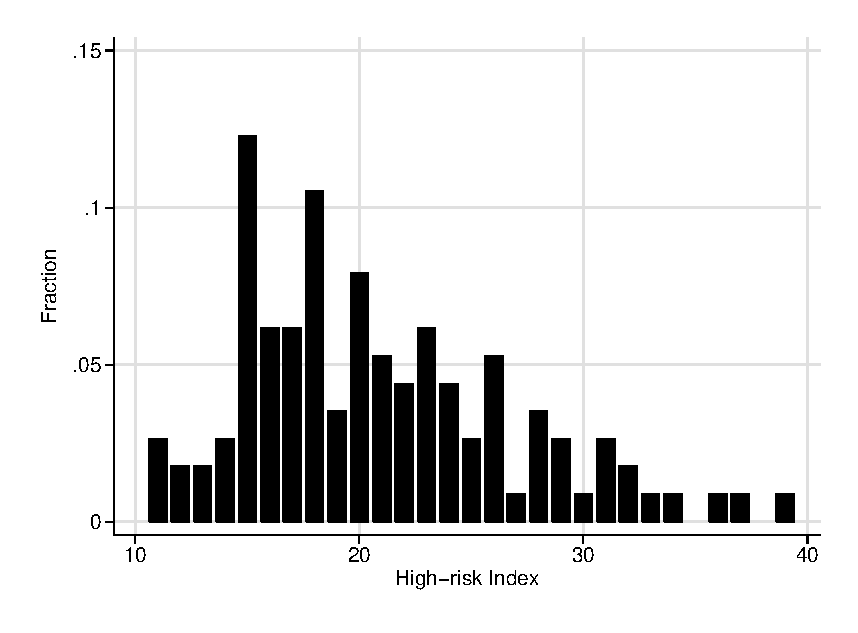
\includegraphics[width=.9\columnwidth]{output/abc_hri.eps}
\floatfoot{
\footnotesize
\noindent Note: This plot shows the distribution of the High-risk Index (HRI) for ABC, which determined eligibility. Subjects were eligible if they had a score of 11 or more.}
	\end{figure}
\end{center}

\begin{center}
	\begin{figure}[H]
		\caption{High-risk Index Distribution, CARE} \label{figure:hridistcare}
		\centering
		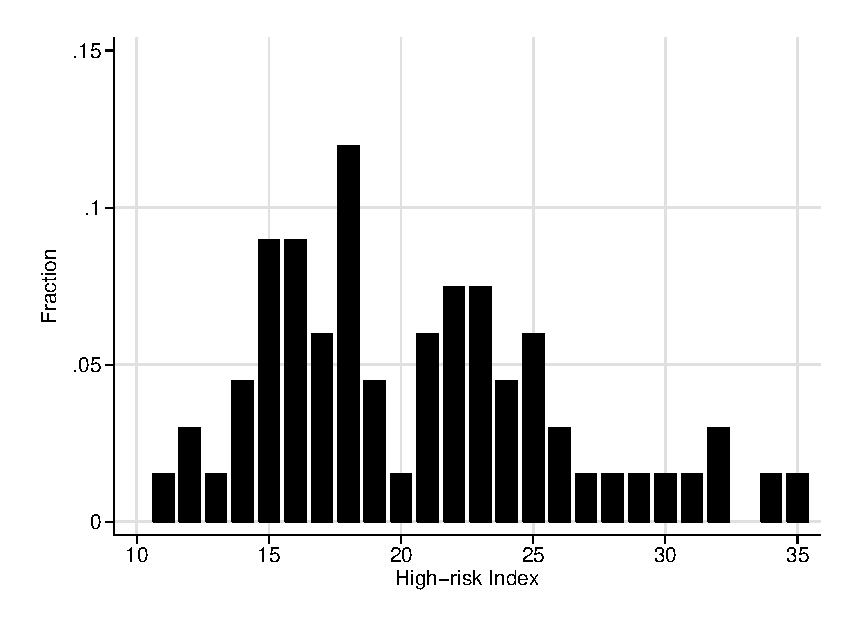
\includegraphics[width=.95\columnwidth]{output/care_hri.eps}
\floatfoot{
\footnotesize
\noindent Note: This plot shows the distribution of the High-risk Index (HRI) for CARE, which determined eligibility. Subjects were eligible if they had a score of 11 or more.}
	\end{figure}
\end{center}


\subsection{Randomization Protocol and Compromises} \label{appendix:randomization}

\noindent Randomization compromises throughout ABC's and CARE's implementations pose a challenge when evaluating the programs' effects. We discuss each case of compromise in detail. Figure~\ref{fig:abc-flow} and Figure~\ref{fig:care-flow} are flow charts that depict the sample from the first-phase randomization through the last data follow-up accounting for all cases of attrition and non-compliance.\\

\noindent Although most randomization compromises occurred at early stages, this methodology also accounts for the fact that a few subjects were not in the sample either for the second-phase randomization or for the adult follow-ups. In Appendix~\ref{appendix:data}, we describe the sample reductions that attrition at different stages of the study generates and test potential differences between the subjects who completed data follow-ups and the subjects who did not.\\

\newgeometry{top=.1in, bottom=.1in, left=.1in, right=.1in}
	\begin{figure}[H]
		\caption{Randomization Protocol and Treatment Compliance, ABC} \label{fig:abc-flow}
		\centering
		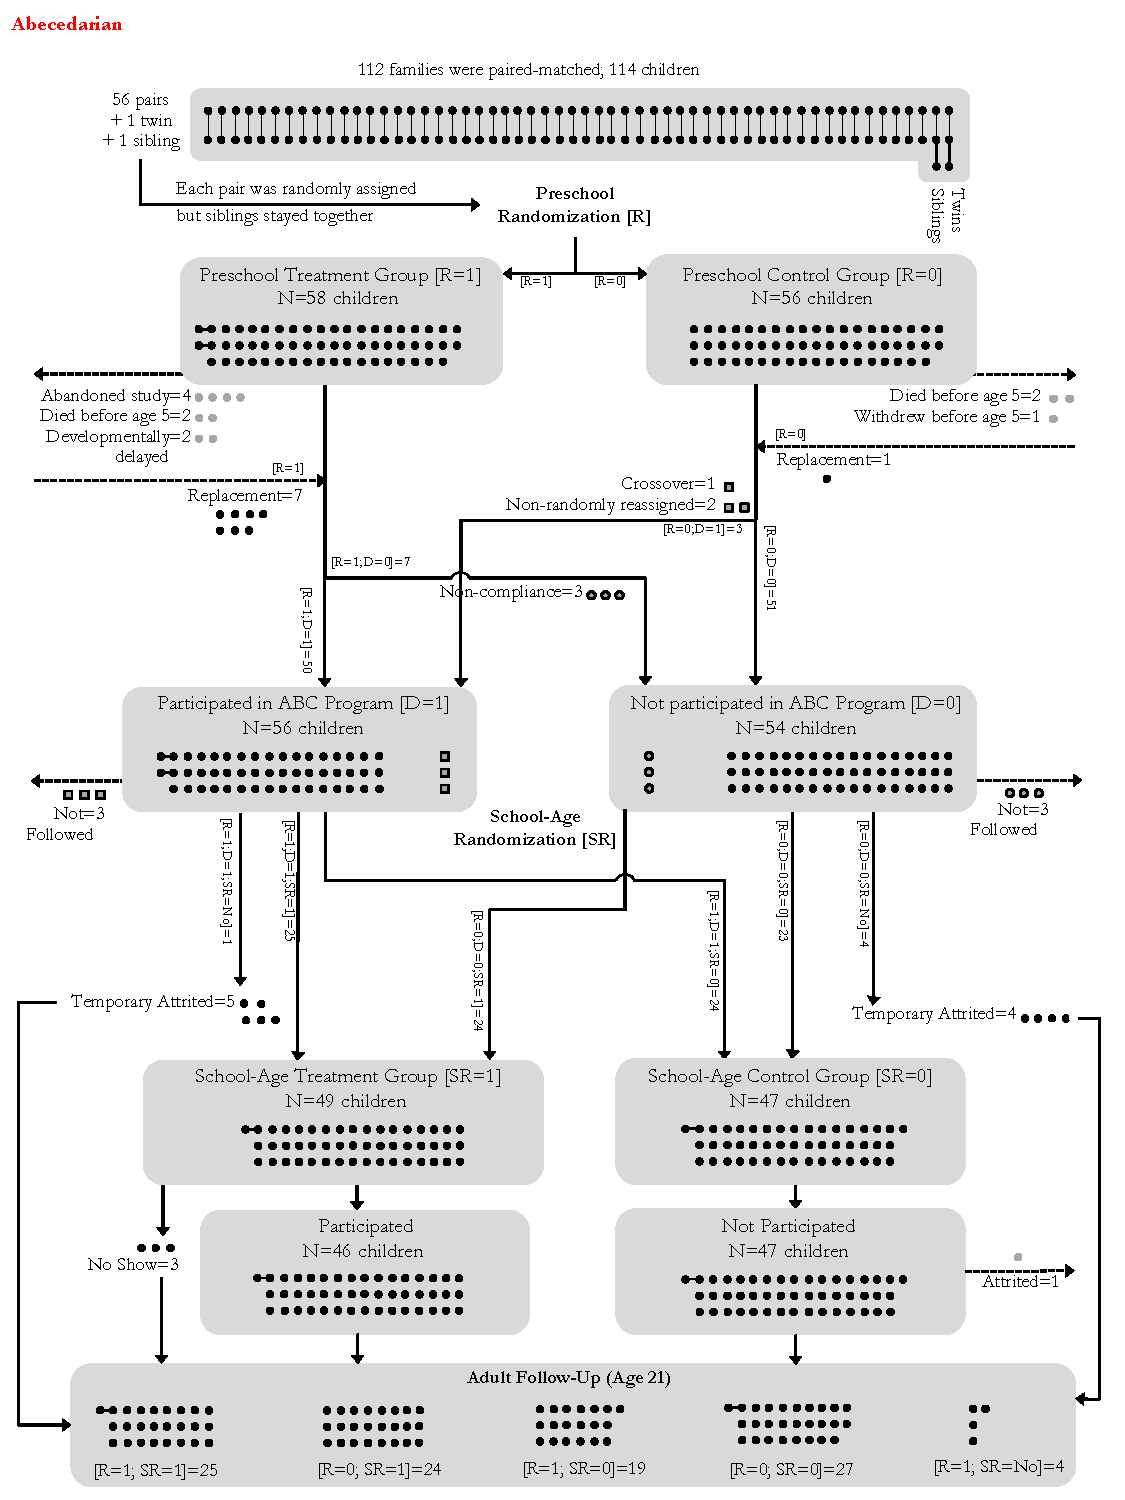
\includegraphics[width=.92\columnwidth]{output/abc_Diagram.pdf}
	\end{figure}
	
	\begin{figure}[H]
		\caption{Randomization Protocol and Treatment Compliance, CARE} \label{fig:care-flow}
		\centering
		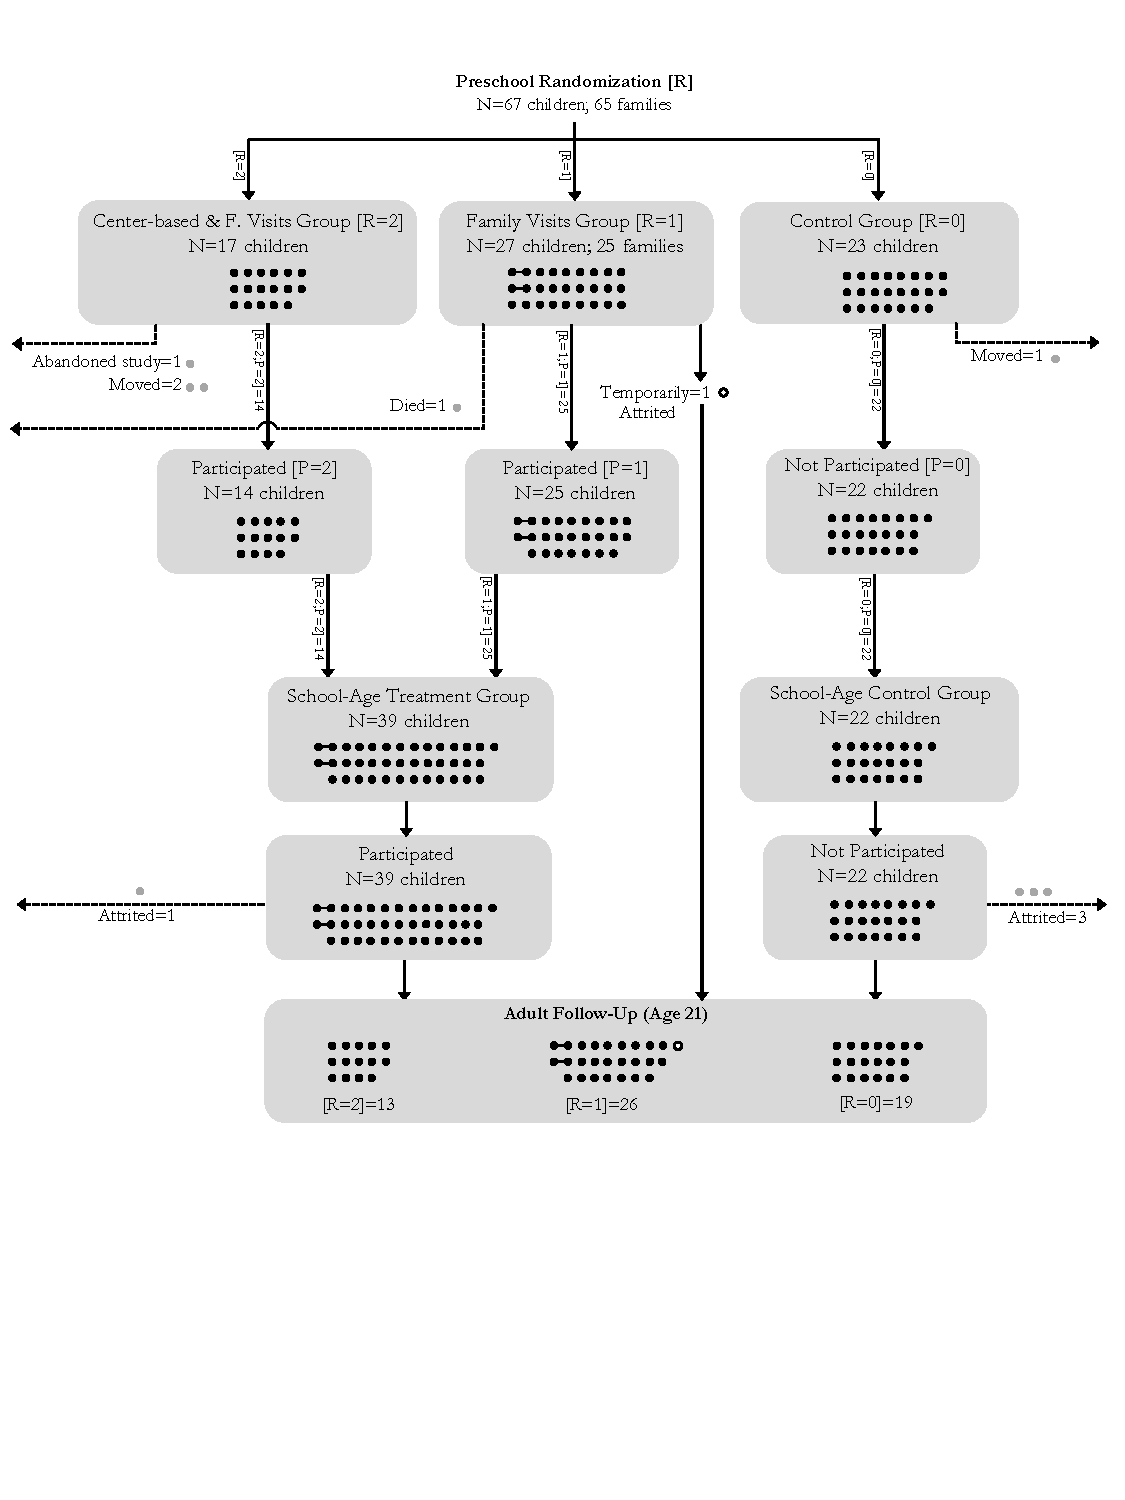
\includegraphics[width=.92\columnwidth]{output/care_Diagram.pdf}
	\end{figure}
\restoregeometry

\doublespacing

\noindent \textbf{Details on Figure~\ref{fig:abc-flow}:} Sources: \cite{Ramey_Collier_etal_1976_CarolinaAbecedarianProject, Ramey_Smith_1977_AJMD,Ramey_Campbell_1979_SR,Ramey_Campbell_1984_AJMD}, internal documentation of the program, and own calculations. Note: The variable $R$ represents randomization into treatment, $[R=1]$, or control, $[R=0]$, groups. After the original randomization, some subjects died or withdrew from the program early in life and were replaced. $R$ also includes those replacements. Arrows pointing outside of the diagram indicate subjects who left the study permanently. The variable $D$ represents participation in the preschool-age program. The variable $SR$ represents randomization into the school-age program, $[SR=1]$, or out of it, $[SR=0]$. Some subjects were not randomized at school age, $[SR=No]$. We use the term ``temporarily attrited" for subjects who did not participate in the study at school age, but were later interviewed in the age-21 followup. \\

\noindent \textbf{Details on Figure~\ref{fig:care-flow}:} Sources: \cite{Wasik_Ramey_etal_1990_CD}, internal documentation of the program, and own calculations. Note: The variable $R$ represents randomization into center-based childcare and family education, $[R=2]$, family education, $[R=1]$, or control, $[R=0]$. Arrows pointing outside of the diagram indicate subjects who left the study permanently. The variable $D$ represents participation in the corresponding group of the preschool-age program. The variable $SR$ represents those who participated in the school-age program, $[SR=1]$, or did not, $[SR=0]$. Unlike in ABC, there was no second-phase randomization in CARE. Rather, those in the center-based childcare and family education group and those in the family education group were automatically assigned to receive the school-age treatment. We use the term ``temporarily attrited" for subjects who did not participate in the study at school age, but were later interviewed in the age-21 followup.

\subsubsection{ABC}

\noindent Both the first and second phases of randomization were conducted at the family level, so pairs of siblings and twins were jointly randomized into either treatment or control groups.\footnote{Sibling pairs occurred when the two siblings were close enough in age such that both of them were eligible for the program.} Although we know that pairing was based on HRI, maternal IQ, maternal education, maternal age, and gender of the subject, we do not know the original pairs. The study collected an initial sample of 120 families. Twenty-two subjects did not complete the first-phase of treatment as initially assigned by the randomization (see Table~\ref{table:abccompromises}).\footnote{In Appendix~\ref{appendix:methodology}, we compare the observed baseline characteristics of the subjects in Table~\ref{table:abccompromises} to the observed baseline characteristics of the subjects who complied to the initial treatment assignment. We find little evidence of differences.}\\


\noindent Of these cases, there were four subjects assigned to treatment who left the study before any data on them was collected. In our main methodology, we assume that they are missing at random. \\

\noindent Second, four subjects died before age 5---two of them initially assigned to treatment and two of them initially assigned to control. For all of them, we observe baseline characteristics and any other data collected before their death. For methodological purposes, they represent cases of program attrition when we do not observe their outcomes.\\

\noindent Third, three subjects in the treatment group did not comply to treatment status. They are different from the four subjects who left the study before any data collection because we observe data collected for them from birth to age 8. Afterward, the program staff chose not to follow them anymore.\footnote{Informal conversations with the program's staff do not indicate a clear reason for this.} Therefore, these subjects remain in treatment sample until age 8 or before. After, they represent cases of program attrition, given that we do not observe them anymore.\\

\begin{sidewaystable}[H] 
\begin{threeparttable}
\caption{Randomization Compromises, ABC}
\label{table:abccompromises}
\centering
\footnotesize
\begin{tabular}{ccccc} \toprule
Child ID & Initial Assignment & Compromise Description & Data Availability & Methodology Assumption \\ \\ \midrule
Case A & Treatment & Left the study & None & Missing at random \\
Case B & Treatment & Left the study & None & Missing at random \\
Case C & Treatment & Left the study & None & Missing at random \\
Case D & Treatment & Left the study & None & Missing at random \\ \midrule
.x    & Control  & Died (age 0), heart disease & Baseline; before dead & Attrition after death \\
914 & Control  & Died (age 0), heart disease & Baseline; before dead & Attrition after death \\
74 & Treatment & Died (age 0), SIDS & Baseline; before dead & Attrition after death \\
99 & Treatment  & Died (age 4), pedestrian accident & Baseline; before dead & Attrition after death \\ \midrule
900 & Treatment  & Non-compliance  & Baseline; before age 8 & Attrition after age 8  \\
912 & Treatment  & Non-compliance  & Baseline; before age 8 & Attrition after age 8  \\
922 & Treatment  & Non-compliance  & Baseline; before age 8 & Attrition after age 8  \\ \midrule
78  & Control        & Crossover from control to treatment & Baseline; before age 8 & Attrition after age 8  \\ \midrule
85 & Treatment   & 3 months of treatment &  Baseline; after age 2 & Same as treatment group  \\  
103 & Treatment &10 months of treatment &  Baseline; after age 2 & Same as treatment group  \\
108 & Treatment & 6 months of treatment &  Baseline; after age 2 & Same as treatment group  \\ 
123 & Treatment & 9 months of treatment &  Baseline; after age 2 & Same as treatment group  \\  \midrule
906 & Control  & Left study at 54 months & Baseline; before 54 months & Attrition after 54 months \\ \midrule
95   & Treatment       & Developmentally delayed at 6 months & No data after diagnosis & Dropped (non-eligible) \\ 
124 & Treatment       & Developmentally delayed at 36 months & No data after diagnosis & Dropped (non-eligible) \\ \midrule
 82 & Control       & Crossover from control to treatment & Baseline, before age 8 & Dropped (non-eligible)  \\ 
 119 & Control       & Crossover from control to treatment & Baseline, before age 8 & Dropped (non-eligible)  \\ \bottomrule
\end{tabular}
\begin{tablenotes}
\item Note: This table describes the various randomization compromises in ABC. For each child, we display: the ID assigned by the program staff, the nature of the compromise, the data available, and the methodological assumption when accounting for non-compliance and program attrition. 
\end{tablenotes}
\end{threeparttable}
\end{sidewaystable}

\noindent Fourth, one subject initially assigned to control was enrolled into treatment. The mother wanted to work and the program staff decided to admit her child into center-based care.\footnote{Correspondence with the program officers stating this permission is available under request from the authors.} Both in terms of data collection and in terms of methodological purposes, this subject is analogous to the subjects in the third case.\footnote{The sensitivity analysis finding little evidence when adjusting for non-compliance includes this case.}\\

\noindent Fifth, four subjects in the treatment group did not complete treatment in its entirety. They were treated for at most 10 months. Except for follow-ups during childhood, which our main results do not use, we observe most of the data for these subjects. We avoid taking a stance on how beneficial the program was at each age, because we do not have a way to document this. Therefore, we assume that they were treated as other subjects in the treatment group.\footnote{If anything, this downward biases the effects of the program we estimate.} \\

\noindent Sixth, the family of one subject in the control group moved at age 54 months. We observe data before the family moved, so we consider the subject as part of the control group in any estimation before this event. Afterwards, we do not observe any data on the subject, so we consider her a case of program attrition.\\

\noindent Seventh, two subjects initially assigned to treatment status were diagnosed as developmentally delayed after 6 and 36 months of treatment. No data for them are available after the diagnosis. We drop them from the sample because they were not eligible to be part of the program.\\

\noindent Finally, two subjects initially assigned to the control group were admitted into treatment. Local authorities requested this because the children were considered highly at risk. Data on them are available from birth to age 8. Although they crossed over from the control group to the treatment group, we consider them to be members of the control group who attrited after age 8.\\

\noindent Analysis of each of these cases leads to the following conclusions. For four subjects, we do not have data to assess them as cases of program attrition, though sensitivity analyses suggest that the treatment effects of the program persist after assigning them the same outcome as the subjects who did the worst in the treatment group. For the subjects who did not comply to treatment, adjusting our estimates for non-compliance when data are available makes little difference. The remaining 14 subjects who did not complete treatment as initially assigned represent various cases of program attrition, for which we propose a correction methodology in Appendix~\ref{app:method_partialobs}.\\

\noindent To increase the number of subjects in the sample, the program officers recruited additional subjects who were added to the program before the subjects were 6 months old. Our calculations indicate that there were eight replacements. We cannot distinguish in the data the subjects who were initially randomized from the replacement children and there is no documentation on how these subjects were recruited.\footnote{Three replacements are reported in \citet{Ramey_Campbell_1979_SR}. Three are documented in correspondence with the program officers, which is available from the authors upon request. The other two replacements are implied by the number of subjects who participated in the randomization protocol in each cohort.} After the various compromises, the sample consisted of 111 subjects: 53 in the treatment group and 58 in the control group. The observed characteristics for each subjects indicate that they were eligible for the program; all subjects in the sample have an HRI of 11 or above. \\

\noindent Prior to the second phase of randomization, 3 subjects in the first-phase control group and 3 subjects in the first-phase treatment group could not be located for follow-up. One subject in the control group and eight subjects in the treatment group of the first phase did not participate in the second phase but later agreed to participate in the data collections during adulthood. This yielded a sample of 96 subjects in the second phase: 49 in treatment and 47 in control. After the second-phase randomization, three subjects in the treatment group chose not to participate in the program, while all subjects in the control group adhered to their randomization status. \\

\subsubsection{CARE}

\noindent The randomization protocol in CARE had no major compromises.\footnote{\citet{Wasik_Ramey_etal_1990_CD,Burchinal_Campbell_etal_1997_CD}.} Of the 65 initial families, 23 were randomized to a control group, 25 to the family education treatment group (we do not consider this group in our combined ABC/CARE sample), and 17 to the family education and center-based childcare treatment group. Two families in the family education treatment group had twins who were jointly randomized, as in ABC. We document four cases of program attrition (see Table~\ref{table:care_compromises}).\footnote{In Appendix~\ref{appendix:methodology}, we compare the observed baseline characteristics of the subjects in Table~\ref{table:care_compromises} to the observed baseline characteristics of the subjects who complied to the initial treatment assignment. We find little evidence of differences.} For methodological purposes, we consider these subjects analogous to their corresponding cases in ABC. We do not present exercises to evaluate the sensitivity to non-compliance because there was none in CARE. Figure~\ref{fig:care-flow} illustrates CARE's randomization protocol and the presence of subjects throughout the data follow-ups.\\

\begin{sidewaystable}[H] 
\begin{threeparttable}
\caption{Randomization Compromises, CARE}
\label{table:care_compromises}
\centering
\footnotesize
\begin{tabular}{ccccc} \toprule
Child ID & Initial Assignment & Compromise Description & Data Availability & Methodology Assumption \\ \\ \midrule
310 & Family education & Died (age 0), unknown causes & Baseline & Attrition after dead \\
301 & Center-based Childcare and Family Education  & Left study at age 5  & Baseline; before age 5 & Attrition after age 5 \\
910 & Control & Move at 11 months old & Baseline; before 11 months & Attrition after 11 months \\
142 & Center-based Childcare and Family Education & Move at 5 months old & Baseline; before 5 months & Attrition after 5 months \\
150 & Center-based Childcare and Family Education & Move at age 5 & Baseline; before age 5 & Attrition after 5 \\ \bottomrule
\end{tabular}
\begin{tablenotes}
\item Note: This table describes the various randomization compromises in CARE. For each child, we display: the ID assigned by the program staff, the nature of the compromise, the data available, and the methodological assumption when accounting for non-compliance and program attrition. 
\end{tablenotes}
\end{threeparttable}
\end{sidewaystable}


\subsection{Program Description and Content}

\subsubsection{Goals}
\noindent The original goals of treatment were to prevent mental retardation by enhancing overall development from birth, in turn fostering school-readiness for an at-risk population.\footnote{Note that the clinical understanding of mental retardation was once associated with disadvantages that hindered early-life development \citep{Mental-Retardation_America_2004_BOOK_NYU}.} Additional curriculum goals were to (i) support language, motor, and cognitive development; (ii) minimize high-risk behaviors; and (iii) develop socio-emotional competencies considered crucial for school success including task-orientation, communicative competence, independence, and prosocial behavior.\footnote{\citet{Ramey_Collier_etal_1976_CarolinaAbecedarianProject, Ramey_etal_1985_Project-CARE_TiECSE, Sparling_1974_Synth_Edu_Infant_SPEECH, Wasik_Ramey_etal_1990_CD, Ramey-etal_2012-ABC}.} Implementation of ABC's and CARE's educational treatments evolved each successive year as program staff evaluated ongoing outcome data.\footnote{ \citet{Ramey-etal_1975_AJoMD, Finkelstein_1982_Day_Care_YC, McGinness_1982_Language-Poverty-Child,Haskins_1985_CD}.}\\


\subsubsection{Daily Schedule}
\noindent For both ABC and CARE, FPGC was open to families from 7:45 a.m. to 5:30 p.m., 5 days per week and 50 weeks per year.\footnote{\citet{Ramey_Collier_etal_1976_CarolinaAbecedarianProject, Ramey_etal_1985_Project-CARE_TiECSE}.} Subjects were offered free transportation to and from the center. A driver and second adult staffed each vehicle (one van and two station wagons) equipped with child safety seats.\footnote{\citet{Ramey_Campbell_1979_SR,abc2014-2015interviews}.} Approximately 65\% of treated ABC families utilized the free transportation.\footnote{\citet{Barnett_Masse_2002_benefitcost}.} Vehicles typically arrived by 9:00 a.m. to the center and departed around 3:45 p.m.\footnote{\citet{Ramey-et-al_1977_Intro-to-ABC}.} At FPGC, ABC and CARE treatment-group subjects received breakfast, lunch, and a snack planned by a nutritionist.\footnote{ \citet{Haskins_1985_CD, Bryant_et_al_1987_Carolina_Approach_TIECSE, Ramey-et-al_1977_Intro-to-ABC}.} Meals were catered by off-site kitchens. Infants received iron-fortified formula  until doctors advised adding solid food. The control-group subjects also received an unlimited amount of iron-fortified formula until approximately 15 months of age.\footnote{\citet{Campbell_Conti_etal_2014_EarlyChildhoodInvestments,abc2014-2015interviews}.}\\

\subsubsection{Program Staff and Physical Space}
\noindent To promote trust in FPGC within the subjects' families, staff were recruited from the local community.\footnote{\citet{Ramey-et-al_1977_Intro-to-ABC, Bryant_et_al_1987_Carolina_Approach_TIECSE, Feagans_1996_Childrens-Talk,abc2014-2015interviews}.} Infant and toddler caregivers and preschool teachers demonstrated varied educational backgrounds ranging from high school graduation to master's degrees. Their average professional working experience with young children was 7 years.\footnote{\citet{Ramey_McGinness_etal_1982_Abecedarianapproach, Ramey_etal_1985_Project-CARE_TiECSE, Wasik_Ramey_etal_1990_CD}.} All classroom staff participated in extensive training and were closely observed by FPGC's academic staff, as part of a broad variety of ongoing clinical and social research related to early childhood education, psychology, and health. In ABC, child-caregiver ratios varied by age: 3:1 for infants up to 13 to 15 months of age; 4:1 for toddlers up to 36 months; and 5:1 or 6:1 for children aged 3 to 5 years, depending on cohort size.\footnote{\citet{Ramey-et-al_1977_Intro-to-ABC,Ramey_Campbell_1979_SR,Ramey_McGinness_etal_1982_Abecedarianapproach}.} Child-caregiver ratios were similar in CARE.\footnote{\citet{Burchinal_Campbell_etal_1997_CD, Ramey_etal_1985_Project-CARE_TiECSE}.}\\

\noindent The ABC and CARE staff included a program director, a secretary, 12 to 14 teachers and assistant teachers, 3 administrative staff members, and a transportation supervisor.\footnote{\citet{Ramey-et-al_1977_Intro-to-ABC,Ramey_McGinness_etal_1982_Abecedarianapproach, Bryant_et_al_1987_Carolina_Approach_TIECSE}.} Lead caregivers and teachers had bachelor's or master's degrees. Teacher aides, recruited from the local community, held high school diplomas (at minimum) and were comparatively well-compensated in the childcare field. They remained a stable treatment component throughout the study. After 1980, following revisions to FIDCR regarding minimum requirements for early childhood education staff, several teacher aides pursued and received undergraduate degrees and became lead teachers. All classroom staff were supervised daily, received weekly mentoring, and professional development from outside consultants..\footnote{\citet{Obrien-Sanders_1974_ABC-brochure, Ramey_etal_1985_Project-CARE_TiECSE, Sanders-Stokes_1979_Status-Report,Klein-Sanders_1982_Status-Report,abc2014-2015interviews}.}\\

\noindent Infant nurseries, toddler rooms, and preschool classrooms were housed on different floors of FPGC. Early reports indicate that FPGC allocated two floors to ABC, but later reports indicate the use of three floors.\footnote{\citet{Ramey_Smith_1977_AJMD,Ramey_Campbell_1979_SR,Ramey_1981_Modification}.} Two infant nurseries were staffed by five adults in a suite of four adjoining rooms: two sleeping rooms contained seven cribs each, while the other two rooms were designated for activities.\footnote{ \citet{Ramey-et-al_1977_Intro-to-ABC}.} The four rooms opened into a large, shared space with feeding tables, an area for food preparation, and a couch.\footnote{\citet{Ramey_Campbell_1979_SR}.} Offices for the medical staff, along with two examining rooms and facilities for laboratory tests were located around the corner from the infant nurseries.\footnote{\citet{abc2014-2015interviews}.} Two multi-age toddler rooms were located one floor below the infant nurseries. One room served children who were 1 to 2 years old and the other served children 2 to 3 years old.\footnote{\citet{Ramey_Smith_1977_AJMD,Ramey_Campbell_1979_SR}.} 3-year-olds were housed in a closed classroom near the toddler rooms. On the lowest floor, 4-year-olds shared an open classroom with a public kindergarten program; the two classes were separated by a long, low bookcase. In CARE, two floors of FPGC were allocated to nurseries and classrooms. A mixed-age classroom design was implemented combining children ages 1 and 3, and children ages 2 and 4. Teacher-child ratios for these ages remained 1:5. FPGC offered two outdoor play areas for both ABC and CARE: one for children up to age 3, and the other for older children.\footnote{\citet{Ramey_Campbell_1979_SR,Ramey_McGinness_etal_1982_Abecedarianapproach}.}\\

\subsubsection{Approach to Child Development}
%Direct from the paper
\noindent Curriculum delivery enabled a highly customized learning experience for treated subjects in both ABC and CARE. Infant caregivers recorded child observations on progress charts and collaborated with FPGC's curriculum developers and academic researchers to rotate learning activities every 2 to 3 weeks for each treated subject.\footnote{\citet{Ramey_Collier_etal_1976_CarolinaAbecedarianProject,Campbell_Ramey_1994_CD}.} Preschool rooms featured intentionally organized environments to promote pre-literacy and access to a rich set of learning tools. The full-day curriculum emphasized active learning experiences, dramatic play, and pre-academics. Frequent 1:1 or 2:1 child-adult interactions prioritized language development for social competence. For ages 3 through 5, as the cohorts approached public school entry, classroom experiences were increasingly structured  towards the development of pre-academic skills and ``socio-linguistic and communicative competence.''\footnote{\citet{Ramey-et-al_1977_Intro-to-ABC, Haskins_1985_CD, Ramey_1981_Modification, Ramey_Campbell_1979_SR, Ramey_Smith_1977_AJMD, Ramey_McGinness_etal_1982_Abecedarianapproach, Sparling_Lewis_1979_BOOKLearninggamesFirstThree,Sparling_Lewis_1984_BOOKLearningGamesThreesFours}.} FPGC offered a summer program before the start of kindergarten designed to target specific skills to ensure success in a kindergarten classroom (e.g., lining up when exiting the classroom). This program was available to subjects in both the center-based childcare and family education group and the family education group.\footnote{\citet{Ramey_etal_1985_Project-CARE_TiECSE}.} \\

\noindent ABC's and CARE's learning programs were influenced by key developmental theorists.\footnote{These include including Bowlby, Piaget, and Vygotsky. \citep{Sparling_1974_Synth_Edu_Infant_SPEECH,Mcginness_1981_Developing,abc2014-2015interviews}.} All four ABC cohorts and two CARE cohorts participated in curriculum developers Sparling and Lewis' ``LearningGames for the First Three Years.''\footnote{ \citet{Sparling_Lewis_1979_BOOKLearninggamesFirstThree}.} The ``LearningGames'' were implemented daily by infant and toddler caregivers in 1:1 child-adult interactions. Each ``LearningGames'' activity stated a developmentally-appropriate objective, the necessary materials, directions for teacher behavior, and expected child outcome. The activities were designed for use both indoors and outdoors, while dressing, eating, bathing, or during play.\footnote{\citet{Ramey_Campbell_1979_SR, Ramey_1981_Modification,Sparling_Lewis_1979_BOOKLearninggamesFirstThree}.}\\

\noindent Supplemental curricula for preschool rooms varied throughout the study, and included ``Cook and Learn,'' ``Peabody Early Experiences Kit,'' ``GOAL Math Program,'' and ``My Friends and Me.''\footnote{ \citet{Greenberg_Epstein_1973_BOOKBridgestoreading,Karnes1973,Dunn_Chun_etal_1976_BOOKPeabodyearlyeducation,Davis_1977_BOOKMyfriends,Wallach_1976_Teaching-All-Children}.}
%SK notes to co-authors: I'm currently waiting for info from Lynne Vernon-Feagans to potentially include a social worker to the list of staff!

\noindent CARE subjects randomized into the center-based childcare and family education group or the family education group also received home visits designed to transmit information on child development and skills involved with parenting including strategies for parent-child interactions based on ``LearningGames" activities and problem-solving techniques.\footnote{\citet{Bryant_et_al_1987_Carolina_Approach_TIECSE, Wasik_Ramey_etal_1990_CD, Burchinal_Campbell_etal_1997_CD}.} Home visitors were trained to ensure they were able to form a strong relationship with the parent and successfully implement the curriculum.\footnote{\citet{Bryant_et_al_1987_Carolina_Approach_TIECSE}.} The visits lasted about an hour, and occurred weekly until the child was 3 years old. After age 3, the home visits were less frequent and depended on the preferences of the parents. They were usually about once a month after age 3.\footnote{\citet{Bryant_et_al_1987_Carolina_Approach_TIECSE, Wasik_Ramey_etal_1990_CD, Burchinal_Campbell_etal_1997_CD}.} \\

\subsubsection{Medical Care and Nutrition}
%Direct from the paper
ABC and CARE provided comprehensive on-site medical care because it was conducted in conjunction with a longitudinal medical research study on infectious respiratory diseases in group environments.\footnote{\citet{Henderson-et-al_1982_NEJoM}.} Treatment group children were monitored daily for signs of illness. All treated children received medical care while attending center-based childcare; the first ABC cohort of control-group children also received medical care during the program's first year of implementation.\footnote{\citet{Ramey_Collier_etal_1976_CarolinaAbecedarianProject, Bryant_et_al_1987_Carolina_Approach_TIECSE, Ramey_Campbell_1991_childreninpoverty,Campbell_Ramey_1994_CD}.}$^{,}$\footnote{Subjects in both the treatment and control groups of the first cohort received free medical care provided by ABC. The control group of the first cohort only received medical care in the first year of the program; the treatment group of the first cohort received medical care for all years of the program. In the subsequent cohorts, only subjects in the treatment group received free medical care provided by ABC. Both CARE cohorts of treated subjects received medical care.}\\
%Direct from the paper

\noindent In ABC, primary pediatric care was provided by a family nurse practitioner and a licensed practical nurse, both under the supervision of one pediatrician who was on continuous duty at the center.\footnote{\citet{Haskins-et-al_1978_JoPP}.} In CARE, the medical staff included two pediatricians, a family nurse practitioner, and a licensed practical nurse.\footnote{\citet{Bryant_et_al_1987_Carolina_Approach_TIECSE}.} The medical staff provided regularly scheduled check-ups, immunizations, parental counseling, and initial assessment of illnesses.\footnote{\citet{Ramey-et-al_1977_Intro-to-ABC, Bryant_et_al_1987_Carolina_Approach_TIECSE}.} The treatment group received standard check-ups when they were 2, 4, 6, 9, 12, 18, and 24 months old and annually thereafter. While in treatment, they also received the standard immunizations.\footnote{\citet{Bryant_et_al_1987_Carolina_Approach_TIECSE, Campbell_Conti_etal_2014_EarlyChildhoodInvestments}.} In ABC, a licensed practical nurse visited classrooms for up to two hours on a daily basis to monitor the subjects' health status.\footnote{\citet{Sanyal_Henderson_etal_1980_JoPediatrics}.} Although this medical care was offered to the treatment-group families free of charge, it was the policy of the medical staff to refer families to a community hospital for serious treatment. While ABC and CARE provided aspirin, immunizations, and basic medicines, families were responsible for purchasing any prescription medication subjects required. There are no data currently available on treatment received for serious conditions or use of prescription medication.  \\

\noindent Infants were supplied with iron-fortified formula. Children older than 15 months of age were provided breakfast, lunch, and an
afternoon snack all planned by a nutritionist.\footnote{\citet{Bryant_et_al_1987_Carolina_Approach_TIECSE, Campbell_Conti_etal_2014_EarlyChildhoodInvestments,abc2014-2015interviews}.} Control families received diapers for up to three years and unlimited iron-fortified bottled formula through 15 months.\footnote{\citet{Ramey_Collier_etal_1976_CarolinaAbecedarianProject,Ramey_Campbell_1979_SR, Ramey_etal_1985_Project-CARE_TiECSE}.}

\subsubsection{School-age Treatment}

\noindent The ABC subjects were randomization into a second-phase, school-age treatment (95 subjects continued to this stage of treatment). The CARE subjects in the center-based childcare and family education group and the family education group received the school-age treatment without randomization. The school-age treatment lasted for the first three years of elementary school and consisted of home visits conducted by a Home/School Resource Teacher.\footnote{\cite{Burchinal_Campbell_etal_1997_CD}.} These visits were structured to increase exposure to reading and mathematics and promote parental involvement in the academic process.\\

\noindent The curriculum was delivered through sets of activities that developed skills such as handwriting, phonics, and math facts.\footnote{There were about 60 activities per year. See \cite{Campbell-Ramey_1989_Preschool-vs-School-age} for details.} Teachers worked to encourage parental involvement in the subjects' academics and provided incentives to families to comply with the treatment, such as giving gift certificates to restaurants and books for the subjects upon the completion of activity packets. \\

\noindent Teachers had graduate-level education, training in special education, \textit{or} were qualified to act as consultants for in-school teachers to address any problems that arose.\footnote{\cite{Ramey_Campbell_1991_childreninpoverty}.} They met with parents at home and with teachers in the schools to deliver new activities for the parents to complete with their children and discuss the child's level of success with the previous set of activities. In addition, they helped parents with issues such as adult literacy, housing, and medical care. Thus, the teacher had a dual role as a parent educator and an advocate for the subject in their educational institution.

\subsection{Control Group Substitution}\label{app:control-subbb}

\noindent In ABC, the families of $75\%$ of the control-group subjects enrolled their children in alternative center-based childcare. In CARE, $74\%$ of families in the control group and $62\%$ of families in the family education group enrolled their children in alternative center-based childcare. We refer to this phenomenon as control substitution; accounting for it is fundamental when evaluating the program.\footnote{See \cite{Heckman_1992_randomization}, \cite{Heckman_2001_EJ}, and \cite{Kline_Walters_2016_QJE}.} In this Appendix, we thoroughly describe the characteristics and costs of the childcare centers providing alternative treatment, in order to create a comparison with the treatments offered by ABC and CARE.\\

\noindent Most of the families in the ABC and CARE control groups enrolled their children in alternative preschool that received federal subsidies and, therefore, were regulated. Figure~\ref{fig:ccabc} and Figure~\ref{fig:cccare} show the amount of enrollment into subsidized and non-subsidized care for ABC and CARE, respectively. Subsidized centers were required to have trained staff who were able to implement curricula designed to enhance cognitive, social, and linguistic competence in disadvantaged children.\footnote{\citet{Burchinal_etal_1989_CD_Daycare-Pre-K-Dev}.} Thus, we consider these centers to offer low-quality center-based childcare. \textbf{[JJH: Jorge, this is not quite consistent with our text--we call all of them low quality] [JLG: You are right and this is outdated. I have updated the sentence.]}

	\begin{figure}[H]
		\caption{Average Number of Months in Alternative Preschool, ABC Control Group} \label{fig:ccabc}
		\centering
		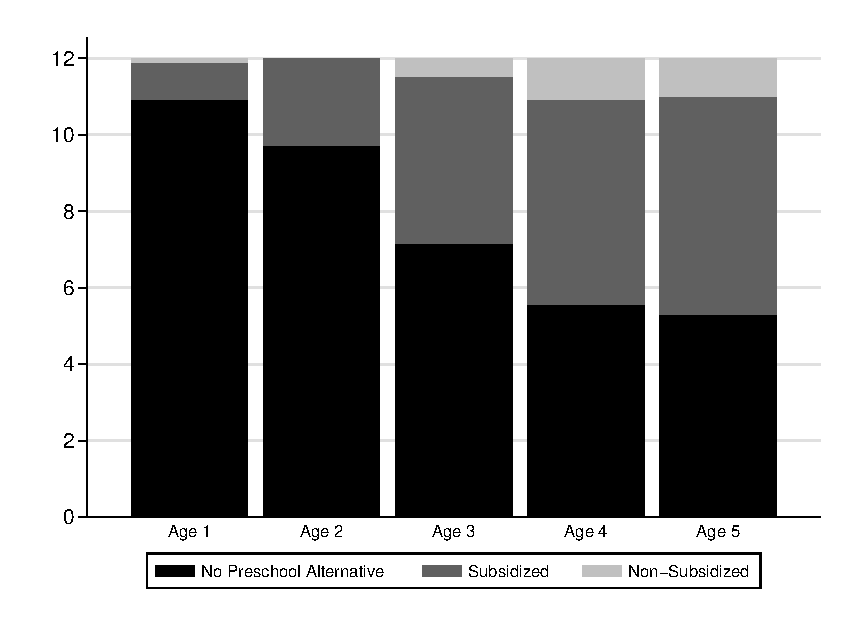
\includegraphics[width=.8\columnwidth]{output/blackwhite_CCnumber.eps}
\floatfoot{
\footnotesize
\noindent Note: This figure describes the take-up of alternative preschool by families in the ABC control group. The vertical axis represents the average number of months per year the subjects of the control group spent in alternative preschool. Subsidized centers were highly regulated and, therefore, relatively high-quality. Non-subsidized childcare services were center-based but not regulated. Other sources of childcare could have included care by parents, relatives, or non-relatives.}
	\end{figure}

	\begin{figure}[H]
		\caption{Average Number of Months in Alternative Preschool, CARE Control and Family Education Groups} \label{fig:cccare}
		\centering
		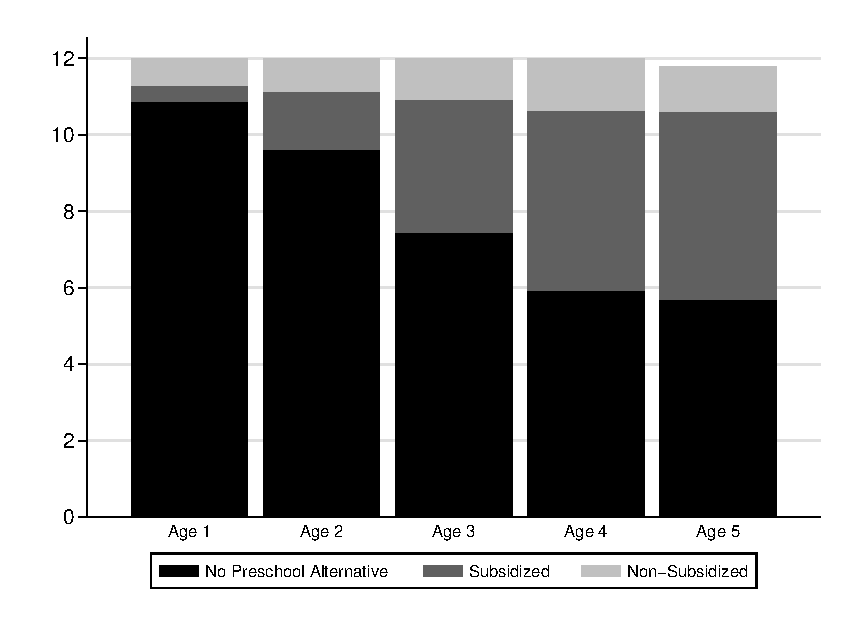
\includegraphics[width=.8\columnwidth]{output/blackwhite_CCnumber_care.eps}
\floatfoot{
\footnotesize
\noindent Note: This figure describes the take-up of alternative preschool by families in the CARE family education and control groups. The vertical axis represents the average number of months per year the subjects of the control group spent in alternative preschool. Subsidized centers were highly regulated and, therefore, relatively high-quality. Non-subsidized childcare services were center-based but not regulated. Other sources of childcare could have included care by parents, relatives, or non-relatives.}
	\end{figure}
	
Table~\ref{table:controlsubscharacteristics} shows baseline characteristics between the control-group subjects who were enrolled in alternative preschool and those who stayed at home. The control-group children who attended alternative preschool were marginally more advantaged, with the most stark difference being maternal employment. This is seen across genders, but is only significant for the female and pooled samples. \textbf{[JJH: What are the treatment effects for high quality versus low quality care?] [JLG: We did try this, but it's honestly impossible to get something useful because the cells get so thin. Even thinner if you consider that we need to split by gender and we have missing information in quality for a third of the sample.]} The males who are enrolled in alternative preschool have mothers with higher IQ scores, but lower parental income indicating lack of spousal support, which is evident by the fewer number of fathers present in that same group. Those who were enrolled in alternative preschools also had more siblings.

\begin{sidewaystable}[H]
\centering
\begin{threeparttable}
\caption{Baseline Characteristics and Control Substitution}\label{table:controlsubscharacteristics}
\begin{tabular}{l c c}
\toprule
Characteristic & \mc{2}{c}{Control Substitution} \\
& No & Yes \\
& $ N=19 $ & $ N=55 $ \\
\midrule
Mother's Yrs. of Edu. &      9.74 &     10.35 \\
                     & (     0.43) & (     0.26)  \\
Mother's Age &     21.42 &     20.27 \\
                     & (     1.79) & (     0.63)  \\
Mother's IQ &     82.00 &     85.60 \\
                     & (     2.32) & (     1.33)  \\
HRI Score &     20.95 &     21.60 \\
                     & (     1.46) & (     0.81)  \\
Number of Siblings &      1.00 &      0.62 \\
                     & (     0.38) & (     0.13)  \\
Male &      0.47 &      0.51 \\
                     & (     0.12) & (     0.07)  \\
Birth Year &   1975.58 &   1975.73 \\
                     & (     0.68) & (     0.32)  \\
Apgar Score, 1 min. &      7.47 &      7.62 \\
                     & (     0.43) & (     0.21)  \\
Apgar Score, 5 min. &      8.63 &      8.98 \\
                     & (     0.26) & (     0.14)  \\
\bottomrule
\end{tabular}
\begin{tablenotes}
\item \footnotesize \textbf{Note:} This table describes baseline characteristics for the children in the control group, by gender and by their enrollment in alternative childcare. The number of subjects in these groups are listed at the top of the table. Asymptotic standard errors are in parentheses. The reported $p$-values are from two-sided tests of difference of means. The means are bolded if the difference is significant at the 10\% level. In the main text, we jointly test for baseline differences between males and females and between treatment- and control-group children, accounting for multiple hypotheses, and find that none of the $p$-values remain significant after this adjustment.
\end{tablenotes}
\end{threeparttable}
\end{sidewaystable}

Figure~\ref{fig:salmonella} shows enrollment by age and the average months of enrollment by age for the control-group children who enrolled in program alternatives. Enrollment increases with the age of children. Figure~\ref{fig:treatsubcare_2} shows the fraction of children enrolled in preschool by age. As control children age, they are more likely to enter childcare.

\begin{sidewaysfigure}[!htbp]
\centering
\caption{Control Substitution Characteristics, ABC/CARE Control Group}\label{fig:control-sub_a}
\begin{subfigure}[h]{0.49\textwidth}
	\centering
	\caption{Enrollment by Age} \label{fig:salmonella}
		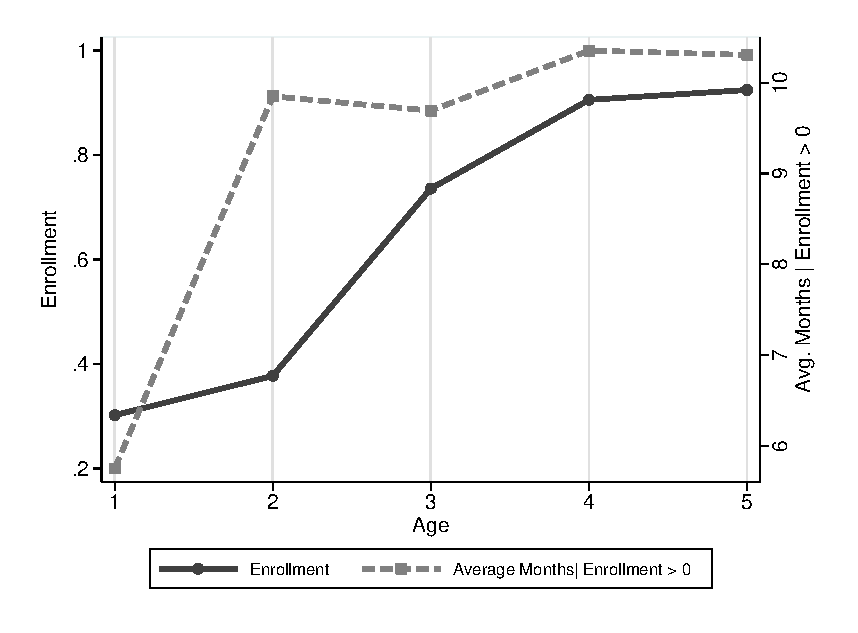
\includegraphics[width=\textwidth]{output/abccare_Valtenrollment.eps}
\end{subfigure}
\begin{subfigure}[h]{0.49\textwidth}
		\centering
		\caption{Enrollment Dynamics} \label{fig:treatsubcare_2}
		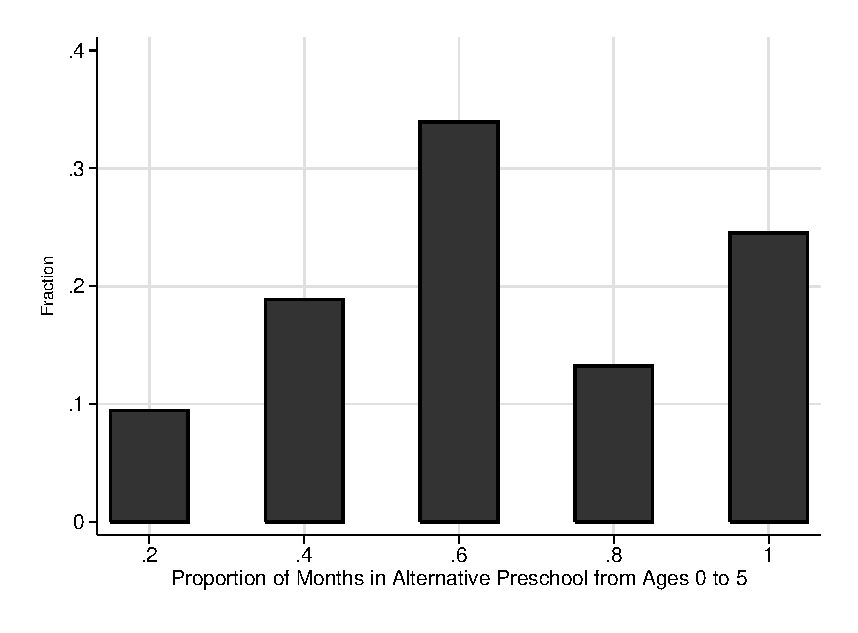
\includegraphics[width=\textwidth]{output/abccare_Vfractimes.eps}
\end{subfigure}%
\footnotesize \justify
Note: Panel (a) displays the fraction of the ABC/CARE control group enrolled in alternatives by age on the left axis and average number of months in alternative preschool by age in the right axis. Panel (b) displays the fraction of children in the ABC/CARE control groups enrolled in alternatives 20\%, 40\%, 60\%, 80\%, and 100\% of the time, from ages 0 to 5.\\
\end{sidewaysfigure}

\subsubsection{Regulation}  \label{appendix:tetanus}

\noindent During the period when both ABC and CARE were active, North Carolina had an active, high-quality system of public childcare for vulnerable families funded by several public programs. Examples include Title IV-A of the Social Service Administration (SSA), Aid to Families with Dependent Children (AFDC), and Title IV-B of Child Welfare Services. These funding efforts were amplified in 1975 by Title XX of the SSA, Social Services Block Grant, which was the main federal source of childcare financing in the U.S. when ABC and CARE were active.\footnote{\citet{Robins_1988_Federal-Child-Care}.}\\

\noindent Federally funded childcare services were regulated according to FIDCR standards, which defined stringent regulation for center-based programs for children between the ages of 3 and 6.\footnote{\citet{Department-of-Health_1968_DayCareRequirements}.} These requirements were enforced.\footnote{\citet{Kuperman_2015_Clifford-Russell-Interview}.} Additionally, North Carolina had a mandatory licensing law for childcare facilities. While FIDCR applied to centers for older children (between the ages of 3 and 6), the North Carolina regulation only applied to centers serving children below the age of 3. The relative weakness of this regulation is not very relevant for our study because treatment substitution occurred mostly after age 3 (see Figure~\ref{fig:ccabc} and Figure~\ref{fig:cccare}).\footnote{\citet{NCGA_1971_House-Bill-100}.} Table~\ref{table:staff} compares a widely-used quality standard, the child-staff ratio, between the North Carolina and FIDCR standards and the actual ABC and CARE numbers. \\

%Not in main paper
\begin{table}[H]
\centering
\caption{Child-Staff Ratios for North Carolina, FIDCR, and Actual ABC and CARE Ratios}
\label{table:staff}
\begin{threeparttable}
\begin{tabular}{lccc}
\toprule
 &NC Standards & FIDCR &  ABC and   \\
Age	& Level I &  Standards  & CARE Ratios\\ \midrule
0--1	& 6:1*	&  				& 	3:1					\\
1--2	& 8:1* 	& 				&   4-5:1				\\
2--3	& 12:1* & 				& 	4-5:1				\\
3--4	& 15:1 	& 		5:1*	& 	4-5:1 				\\
4--5	& 20:1 	& 		7:1*	& 	5-6:1 				\\
5--6 & 25:1  &		7:1*	&	5-6:1				\\
\bottomrule
\end{tabular}
\begin{tablenotes}
\footnotesize
Sources: \cite{Department-of-Health_1968_DayCareRequirements,NCGA_1971_House-Bill-100,Ramey-et-al_1977_Intro-to-ABC,Ramey_Campbell_1979_SR,Ramey_McGinness_etal_1982_Abecedarianapproach, Burchinal_Campbell_etal_1997_CD}.\\
Note: The starred ratios represent the ones we believe were the most relevant for the ABC control-group subjects and the CARE control-group and family-education-group subjects.
\end{tablenotes}
\end{threeparttable}
\end{table}

\textbf{[JJH: Jorge, this is really highly competent]}

\subsubsection{Costs}
% Need citations
\noindent Previous papers have used childcare cost rates that are not specific to North Carolina and do not account for the contemporaneous structure of the subsidies. We use the local subsidy rates that were in place when the ABC subjects were in preschool to impute different costs of the alternative preschools. These costs depend on the specific preschool attended and the eligibility of the families to receive the subsidies. \\

\noindent When ABC and CARE were in operation, center-based childcare was subsidized by several federal programs (the Department of Social Services categorized these programs as Child Welfare, AFDC, and Work Incentive Programs).\footnote{\citet{NC-State-Dept_1972_Licensed-Day-Care}.} However, our calculations of the cost of alternative preschool are simplified by the fact that the subsidies were centralized and regulated by the County Department of Social Services. Those departments used a uniform subsidy rate, regardless of the origin of the funds.\footnote{\citet{Ad-Hoc-NC_1974_Letter}.} We collected information about the subsidy rate at the time, which approximates the price of the centers, as centers pegged their fees and services to the maximum subsidy rate. Moreover, we know which centers each ABC control subject attended. We interviewed North Carolina childcare staff and academics that study childcare to document which of those centers were subsidized and regulated at the time.\footnote{\citet{Kuperman_2015_Clifford-Russell-Interview,Kuperman-Hojman_2015_Hodgers-Interview}.} For subsidized centers, we impute the maximum Department of Social Services fee established at the time: \$633/month in 2014 USD.\footnote{\citet{Ad-Hoc-NC_1974_Letter,Comm-Plan-Serv_1973_Durhams-Share}.} For non-subsidized centers, we impute the mean of costs for Level-1 centers (minimum accepted quality level) according to a 1982 North Carolina study of the cost of childcare: \$298/month in 2014 USD.\footnote{\citet{NC-Admin-Branch_1982_Day-Care-Cost-Study}.} Although the information in this survey is not ideal for assessing the cost of subsidized preschools for CARE, as the subsidies greatly changed after the end of FIDCR (1981), it provides an approximation for assessing the cost of the non-subsidized centers. \\

\noindent Finally, we determine if the families paid the costs themselves or if they were subsidized, in which case we also add deadweight costs. We consider if a subject was eligible for subsidies if the family lived in poverty according to the federal guidelines and all parents living at home worked. If a family is deemed eligible, then we assume the child's preschool was fully subsidized using the rates described above without additional subsidies.\\

\subsection{Data} \label{appendix:data}

In Table~\ref{tab:ecvars_1} through Table~\ref{tab:adultvars_2}, we summarize the data availability for both ABC and CARE. The data collection processes in both programs were analogous by design. For both programs, the treatment and control groups were followed into adulthood with relatively low attrition. For ABC, subjects were followed annually through elementary school and at ages 12, 15, 21, and 30. Health and administrative crime data were collected when the subjects reached their mid-30s. For CARE, the exact same follow-ups are available with the exception of the age 15 follow-up.\\

\begin{sidewaystable}[H]
\small
\caption{Early Childhood Data (Part I)}
\label{tab:ecvars_1}
\centering
\begin{adjustbox}{max width=\textwidth, max height=\textheight,keepaspectratio}
\begin{threeparttable}
\tiny
\begin{tabular}{L{3cm} C{3.5cm} C{4cm} C{1.5cm} C{1.5cm}  C{6cm}}
\toprule
\textbf{Category}	&	\textbf{Sub-Category}	&	\textbf{Description}	&	\textbf{ABC Age}  	&  \textbf{CARE Age}  & 	\textbf{Measure}	\\ \midrule
Demographics	&	Gender	&	Gender of child	&	Birth, 18, 30, 42, 54	&	 Birth, 18, 30, 42, 54	&	Demographic Interview	\\
	&	\\
	&	Race	&	Race/Cultural identity of child	&	Birth, 18, 30, 42, 54	&	 Birth, 18, 30, 42, 54	&	 Demographic Interview\\
	&	\\
	&	Birth Date	&	Date of birth of child	&	Birth, 18, 30, 42, 54	& 	Birth, 18, 30, 42, 54	&	 Demographic Interview	\\ \midrule
Cognitive Assessments	&	Language Ability	&	Auditory association, Verbal expression, etc. 	&	36, 42, 48, 54	&	30, 42, 54	&	ITPA$^{ABC}$, GPB$^{ABC}$, PLP$^{ABC}$, MSCD \\
	&	\\
	&	Intelligence Levels	&	SBIS 	&	24, 36, 48, 60	&	24, 36, 48, 60	&	SBIS	\\
	&		&	WPPSI	&	60	&	60	&	WPPSI	\\
	&		&	BSID 	&	3, 6, 9, 12, 18, 24	&	6, 12, 18, 24		&	BSID	\\
	&		&	UOSPD	&	15	&	- 	&	UOSPD$^{ABC}$	\\
	&		&	RPM	&	60	&	-	&	RPM$^{ABC}$	\\
	&	\\
	&	Quantitative	 &	BSID 	&	3, 6, 9, 12, 18, 24	&	6, 12, 18, 24		&	BSID	\\
	&		&	MSCD 	&	30, 42, 54		&	30, 42, 54	&	MSCD	\\
	&	\\
	&	Memory	&	BSID 	&	3, 6, 9, 12, 18, 24	& 	6, 12, 18, 24		&	BSID	\\
	&		&	MSCD 	&	30, 42, 54	&	30, 42, 54	&	MSCD	\\
	&	\\
	&	Motor Development	&	BSID 	&	3, 6, 9, 12, 18, 24	&	6, 12, 18, 24		&	BSID\\
	&		&	MSCD 	&	30, 42, 54	&	30, 42, 54	&	MSCD	\\
	& 	\\
	&	Critical Thinking	&	Curiosity	&	30, 36, 42, 48, 54, 60, 66, 72	& - &	Infant Behavior Inventory$^{ABC}$	\\ \midrule
Non-Cognitive Assessments	&	Social Skills	&	Positive social response	&	30, 36, 42, 48, 54, 60, 66, 72	&	6, 12, 18, 24		&	Infant Behavior Inventory$^{ABC}$, Bayley Infant Inventory$^{CARE}$	\\
	&		&	Creativity	&	30, 36, 42, 48, 54, 60, 66, 72	&	- 	&	Infant Behavior Inventory$^{ABC}$	\\
	&	\\
	&	Self-Control	&	Locus of control	&	3, 18	&	6, 18	& 	RIES	\\
	&		&	Distractibility, Attentiveness	&	30, 36, 42, 48, 54, 60, 66, 72	&	6, 12, 18, 24		&	Infant Behavior Inventory$^{ABC}$, Bayley Infant Inventory$^{CARE}$	\\
	&	\\
	&	Emotional Health	&	KRT	&	24, 36, 48, 60	&	24, 30, 36, 42, 48, 60	&	KRT	\\
	&	\\
	&	Self-Consciousness	&	Self-consciousness	&	30, 36, 42, 48, 54, 60, 66, 72	&	-	&	Infant Behavior Inventory$^{ABC}$	\\
\bottomrule
\end{tabular}
\begin{tablenotes}
\scriptsize
\item Sources: Authors' description. \\	
\item Note: This table describes the major categories of variables that were measured for ABC and CARE subjects up to age 6. ABC and CARE ages are measured in months. This is not an exhaustive list of variables, nor does it include variables from auxiliary data. Instruments or questionnaires available for only one of the studies are indicated with the superscript $^{ABC}$ or $^{CARE}$.  \textbf{Abbreviations are as follows.} ITPA: Illinois Test of Psycholinguistic Ability. GPB: Gordon Psycholinguistic Battery. PLP: Preschool Language Performance. MSCD: McCarthy Scales of Children's Development. BSID: Bayley Scales of Infant Development and Infant Behavior. UOSPD: Uzgiris-Hunt Ordinal Scales of Psychological Development. RPM: Raven's Progressive Matrices. RIES: Rotter's Internality-Externality Scale. KRT: Kohn and Rosman Test Behavior Inventory.
\end{tablenotes}
\end{threeparttable}
\end{adjustbox}
\end{sidewaystable}




\begin{sidewaystable}[H]
\small
\caption{Early Childhood Data (Part II)}
\label{tab:ecvars_2}
\centering
\begin{adjustbox}{max width=\textwidth, max height=\textheight,keepaspectratio}
\begin{threeparttable}
\tiny
\begin{tabular}{L{3cm} C{3.5cm} C{4cm} C{1.5cm} C{1.5cm}  C{6cm}}
\toprule
\textbf{Category}	&	\textbf{Sub-Category}	&	\textbf{Description}	&	\textbf{ABC Age}  	&  \textbf{CARE Age}  & 	\textbf{Measure}	\\ \midrule
Family Environment	&	Family Members	&	Number of primary caretakers	&	Birth, 18, 30, 42, 54	&	18, 30, 42, 54, 60	&	Demographic Interview	\\
	&		&	Relationship with family members, including father, mother, siblings, etc.	&	Birth, 18, 30, 42, 54	&	18, 30, 42, 54, 60	&	Demographic Interview	\\
	&		&	Number of siblings	&	Birth, 18, 30, 42, 54	&	Birth, 18, 30, 42, 54, 60	&	Demographic Interview	\\
	&		&	Marital status of parents	&	Birth, 18, 30, 42, 54	&	Birth, 18, 30, 42, 54, 60	&	Demographic Interview	\\
	&		&	Marital conflicts between parents	&	6, 18	&	Birth, 6, 18, 36	&	Demographic Interview$^{CARE}$, Parental Attitudes Research Inventory	\\
	&		& Father at home & 18, 30, 42, 54  & 18, 30, 42, 54, 60 & Demographic Interview \\
	&	\\
	&	Family Economic Environment	&	Parents' occupation	&	Birth, 18, 30, 42, 54	& 	Birth, 18, 30, 42, 54, 60		&	Demographic Interview	\\
	&								& Mother works & 18, 30, 42, 54 & 18, 30, 42, 54, 60 & Demographic Interview \\
	&		&	Source of child support	&	Birth, 18, 30, 42, 54	&	18, 30, 42, 54, 60	&	Demographic Interview	\\
	&		&	Family income	&	Birth, 18, 30, 42, 54	&	Birth, 18, 30, 42, 54, 60	&	Demographic Interview	\\
	&	\\
	&	Parents and Home Environment & Parents' authority, warmth, family conflict, etc. & 6, 18, 30, 42, 54 & 6, 12, 18, 30, 42, 54 & Parent Interview \\
	&	\\
	&	Family Social Status	&	Parents' education background	&	Birth, 18, 30, 42, 54	&	Birth, 18, 30, 42, 54, 60		&	Demographic Interview	\\
	&		&	Risk taking of family members	&	Birth	&	- 	&	Parent Interview$^{ABC}$	\\
	&	\\
	&	Family Members' Physical Health	&	Health issues of parents	&	Birth	&	Birth	&	Parent Interview	\\
	&		&	Pregnancy history	&	Birth	&	Birth	&	Parent Interview	\\ \midrule
Childcare	&	Day-care Experience	&	Time and location of day-care, Age when begin	&	Birth, 18, 30, 42, 54	&	18, 30, 42, 54	&	Demographic Interview	\\
			&						& 	Home visits &	-	&	6, 18, 30, 42, 54, 60	& Home Visit Data$^{CARE}$ \\
	&	\\
	&	Parental Care	&	Maternal warmth, Maternal involvement with child	&	6, 18, 30, 42, 54	&	6, 12, 18, 30, 42, 54	&	Home Stimulation	\\
	&		&	Provision of appropriate play materials	&	6, 18, 30, 42, 54	&	 6, 12, 18, 30, 42, 54	&	Home Stimulation	\\
	&		&	Avoidance of restriction and punishment	&	6, 18, 30, 42, 54	&	6, 12, 18, 30		&	Home Stimulation	\\
	&		&	Authoritarian control	&	6, 18, 30, 42, 54	&	6, 12, 18, 30, 36, 42, 102		&	Home Stimulation, Parental Attitudes Research Inventory	\\
	&		&	Democratic attitudes	&	6, 18	&	6, 18, 36	&	Parental Attitudes Research Inventory	\\
	&		&	Hostility and rejection	&	6, 18	&	6, 18, 36	&	Parental Attitudes Research Inventory	\\
	&		&	Parents' knowledge of childcare	&	Birth	&	-	&	Parent Interview$^{ABC}$	\\ \midrule
Physical Health	&	Growth Data	&	Height, Weight, Head circumference, etc.	&	3, 6, 9, 12, 18, 24, 36, 48, 60	&	Birth, 6, 12, 18, 24, 36, 48, 60	&	Growth Measures	\\
\bottomrule
\end{tabular}
\begin{tablenotes}
\scriptsize
\item Sources: Authors' description. \\	
\item Note: This table describes the major categories of variables that were measured for ABC and CARE subjects up to age 6. ABC and CARE ages are measured in months. This is not an exhaustive list of variables, nor does it include variables from auxiliary data.  Instruments or questionnaires available for only one of the studies are indicated with the superscript $^{ABC}$ or $^{CARE}$.
\end{tablenotes}
\end{threeparttable}
\end{adjustbox}
\end{sidewaystable}



\begin{sidewaystable}[H]
\begin{threeparttable}
\small
\caption{Childhood and Adolescence Data (Part I)} \label{tab:youthvars_1}
\centering
\tiny	
\begin{tabular}{L{3.5cm} C{3.5cm} C{5cm} C{1.5cm} C{1.5cm} C{6cm}}
\toprule
\textbf{Category}	&	\textbf{Sub-Category}	&	\textbf{Description}	&	\textbf{ABC Age}  	&  \textbf{CARE Age}  & 	\textbf{Measure}	\\ \midrule
Cognitive Assessment	&	Language Ability	&	Adaptive Language Inventory	&	6, 7, 8	&	6, 7, 8	&	Adaptive Language Inventory	\\
	&		&	Language Questionnaire	&	12	&	- 	&	Language Questionnaire$^{ABC}$	\\
	&		&	MSCD 	&	7	&	- 	&	MSCD$^{ABC}$	\\
	&	\\
	&	Intelligence Tests	&	SBIS	 &	6	&	7	&	SBIS	\\
	&		&	 WIS	&	6, 7, 8, 12, 15	&	6, 8	&	WIS	\\
	&		& Kaufman$^{CARE}$ & 	-	& 6 & Kaufman$^{CARE}$ \\
	&	\\
	&	Quantitative Skills	&	MSCD$^{ABC}$ 	&	7	&	-	&	MSCD$^{ABC}$ 	\\
	&	\\
	&	Memory	&	MSCD$^{ABC}$ 	&	7	&	-	&	MSCD$^{ABC}$	\\
	&	\\
	&	Motor Skills	&	MSCD$^{ABC}$ 	&	7	&	-	&	MSCD$^{ABC}$	\\ \midrule
Non-Cognitive Assessment	&	Interpersonal Skills	&	Gets along with people	&	6, 8, 12, 15	& 	8, 12	&	PEI, CAS, PMI$^{ABC}$, SAI$^{ABC}$, Subject Interview$^{ABC}$, Quality Rank$^{CARE}$	\\
	&		&	Relationship with the other sex	&	15	&	- 	&	 SAI$^{ABC}$, Subject What I Am Like (Harter)$^{ABC}$	\\
	&	\\
	&	Critical Thinking	&	Thinks for self, questions things	&	6, 8	 &	8, 12	&	PEI, Harter Child$^{CARE}$, CBI	\\
	&		&	Concept Attainment Kit	&	6, 7, 8	&	- 	&	Concept Attainment Kit$^{ABC}$	\\
	&	\\
	&	Self-Control	&	Distracted in class	&	6, 7, 8, 12, 15	&	12	&	SCAN$^{ABC}$, CBI, WPB$^{ABC}$, PMI$^{ABC}$, SAI$^{ABC}$, Self-Evaluation Inventory$^{ABC}$	\\
	&		&	Locus of control	&	15	&	- 	&	Nowicki-Strickland Data, Pearlin Mastery Scale$^{ABC}$	\\
	&	\\
	&	Work Ethic	&	Task Orientation	&	6, 7, 8, 12, 15	&	6, 7, 8, 9, 12 	&	SCAN$^{ABC}$, CBI, PMI$^{ABC}$		\\
	&	\\
	&	Emotional Health	&	Harms self, suicidal thoughts	&	8, 12, 15	&	8, 12	 	&	Achenbach Parent,  Subject Risk Taking Survey$^{ABC}$		\\
	&		&	Depression, anxiety, fear, etc.	&	6, 7, 8, 12, 15	&	7, 8, 9, 12	&	KRT, CAS, ETS,  Achenbach Parent	\\
	&	\\
	&	Social Activities	&	Athletic activities	&	8, 12, 15	&	8, 12		&	Achenbach Parent, SAI$^{ABC}$, Subject What I Am Like (Harter)$^{ABC}$, PEI$^{CARE}$	\\
	&		&	Participant of organizations, e.g. religions	&	8, 12, 15	&	8, 12	&	Achenbach Parent, SAI$^{ABC}$, Subject Interview$^{ABC}$	\\
	&		&	Reading list	&	12, 15	&	12	&	CAS, SAI$^{ABC}$	 \\
	&		&	TV/music	&	12, 15	&	12	&	CAS, SAI$^{ABC}$	, Television Checklist$^{ABC}$		\\
	&	\\
	&	Self-Consciousness	&	Self-conscious emotions	&	8, 12, 15	&	8, 12	&	Achenbach Parent, Subject What I Am Like (Harter)	\\ \bottomrule
	\end{tabular}
\begin{tablenotes}
\scriptsize
\item Sources: Authors' descriptions. \\
\item Note: This table describes the major categories of variables that were measured for ABC and CARE subjects at ages 6 to 18. ABC and CARE age are measured in years. This is not an exhaustive list of variables, nor does it include variables from auxiliary data.  Instruments or questionnaires available for only one of the studies are indicated with the superscript $^{ABC}$ or $^{CARE}$. \textbf{Abbreviations are as follows.}  MSCD: McCarthy Scales of Children's Development. SBIS: Stanford-Binet Intelligence Scale. WIS: Wechsler Intelligence Scale for Children. KRT: Kohn and Rosman Test Behavior Inventory. WJCA: Woodcock-Johnson Test of Cognitive Abilities. PEI: Parents as Educator Interview. CAS: Child Assessment Schedule. PMI: Psychosocial Maturity Inventory. SAI: Social Adjustment Inventory for Children and Adolescents. SCAN: Schedule of Classroom Activity Norms. CBI: Classroom Behavior Inventory. WPB: Walker Problem Behavior Checklist. ETS: Emotional/Activity/Sociability/Impulsivity Temperament Survey. FES: Family Environment Scale. PIAT: Peabody Individual Achievement Test. CAT: California Achievement Test. MARS: Mid-Adolescence Rating Scale Data.
\end{tablenotes}
\end{threeparttable}
\end{sidewaystable}

	
	
\begin{sidewaystable}[H]
\begin{threeparttable}
\small
\caption{Childhood and Adolescence Data (Part II)} \label{tab:youthvars_2}
\centering
\tiny
\begin{tabular}{L{3.5cm} C{3.5cm} C{5cm} C{1.5cm} C{1.5cm} C{6cm}}
\toprule
\textbf{Category}	&	\textbf{Sub-Category}	&	\textbf{Description}	&	\textbf{ABC Age}  	&  \textbf{CARE Age}  & 	\textbf{Measure}	\\ \midrule
Family Environment	&	Family Members	&	Number of adults in house	&	6, 8, 12, 15	&	8, 12	&	PEI, Parent Interview, Subject Person In Household$^{ABC}$		\\
	&		&	Relationship with family members, including father, mother, siblings, etc.	&	6, 8, 12, 15	&	8, 12	&	PEI, FES, SAI, Subject Interview$^{ABC}$, Adult Self Report$^{ABC}$, Parent Interview, Achenbach Parent	\\
	&		&	Number of siblings	&	6, 8, 12, 15	&	7, 8, 12	&	PEI$^{ABC}$, Parent Interview	\\
	&		&	Marital status of parents	&	6, 8, 12, 15	&	7, 8, 12	&	PEI$^{ABC}$	, Parent Interview	\\
		&		& Father at home & 18, 30, 42, 54  & 18, 30, 42, 54, 60 & Demographic Interview \\
	&	\\
	&	Parents' Education Style	&	Role of parents in education	&	6, 8	&	8, 12	&	PEI, Parent Interveiw$^{CARE}$	\\
	&		&	Parents' education beliefs \& methods&	6, 8	&	8, 12 	&	PEI, Parent Interview$^{CARE}$		\\
	&		&	Parents' aspiration \& attitudes towards child	&	6, 8, 12, 15	&	8, 12	&	PEI, Parent Interview	\\
	&	\\
	&	Family Economic Environment	&	Parents' occupation	&	6, 8, 12, 15	&	7, 8, 12	&	PEI$^{ABC}$, Parent Interview	\\
		&							& Mother works & 9 & 5, 7, 8 & Demographic Interview \\
	&		&	Source of child support	&	6, 8, 12, 15	&	7, 8, 12	&	PEI$^{ABC}$, Parent Interview	\\
	&		&	Family income	&	6, 8, 12, 15	&	7, 8, 12	&	PEI$^{ABC}$, Parent Interview	\\
	&	\\
		&	Parents and Home Environment & Parents' authority, warmth, family conflict, etc. & 8 & 8 & Parent Interview \\
	&	\\
	&	Family Social Status	&	Parents' education background	&	6, 8, 12, 15	&	7, 8, 12	&	PEI$^{ABC}$, Parent Interview	\\
	&		&	Criminal history and risk taking of family members	&	8, 12, 15	&	- 	&	Subject Taylor Life Events$^{ABC}$, Parent Interview$^{ABC}$	\\
	&	\\
	&	Family Members' Physical Health	&	Health issues of adults in house	&	8, 12, 15	&	12	&	Parent Interview, Subject Taylor Life Events$^{ABC}$	\\ 	\midrule
Academic Achievements	&	Standardized Tests	&	Reading, mathematics, and language abilities	&	6, 7, 8, 12	&	6, 8, 9,12	&	CAT$^{ABC}$, PIAT$^{ABC}$, WJCA	\\
		&	\\
	&	Performance in Schoolwork	&	Drop in grades	&	12, 15		&	12	&	CAS	\\
	&		&	Lack of interest in school	&	12, 15		&	12	&	CAS	\\
	&		&  Total years in special education & 17 & 11 & Retention and Special Services Data \\
	&		&  Total years retained in school & 17 & 11 & Retention and Special Services Data \\  \midrule
Physical Health	&	Health Issues	&	Health issues of subject	&	8, 12, 15	&	8, 12	&	Achenbach Parent, Subject Interview$^{ABC}$, Adult Self Report$^{ABC}$, PEI$^{CARE}$, Parent Interview$^{CARE}$	\\
	&	\\
	&	Growth	&	Vision, weight, height	&	8	&	8	&	Growth Data	\\
	&	\\
	&	Teenage Pregnancy	&	Teenage Pregnancy	&	15	&	- 	& Subject Interview$^{ABC}$		\\ \midrule
Social Conduct	&	Law Breaking	&	Felony, Time spent incarcerated	&	15	&	- 	&	MARS$^{ABC}$, Subject Interview$^{ABC}$	\\ \bottomrule
\end{tabular}
\begin{tablenotes}
\scriptsize
\item Sources: Authors' descriptions. \\
\item Note: This table describes the major categories of variables that were measured for ABC and CARE subjects at ages 6 to 18. ABC and CARE age are measured in years. This is not an exhaustive list of variables, nor does it include variables from auxiliary data.  Instruments or questionnaires available for only one of the studies are indicated with the superscript $^{ABC}$ or $^{CARE}$. \textbf{Abbreviations are as follows.}  MSCD: McCarthy Scales of Children's Development. SBIS: Stanford-Binet Intelligence Scale. WIS: Wechsler Intelligence Scale for Children. KRT: Kohn and Rosman Test Behavior Inventory. WJCA: Woodcock-Johnson Test of Cognitive Abilities. PEI: Parents as Educator Interview. CAS: Child Assessment Schedule. PMI: Psychosocial Maturity Inventory. SAI: Social Adjustment Inventory for Children and Adolescents. SCAN: Schedule of Classroom Activity Norms. CBI: Classroom Behavior Inventory. WPB: Walker Problem Behavior Checklist. ETS: Emotional/Activity/Sociability/Impulsivity Temperament Survey. FES: Family Environment Scale. PIAT: Peabody Individual Achievement Test. CAT: California Achievement Test. MARS: Mid-Adolescence Rating Scale Data.
\end{tablenotes}
\end{threeparttable}
\end{sidewaystable}

\begin{sidewaystable}[H]							
\begin{threeparttable}								
\small										
\caption{Adulthood Data (Part I)} \label{tab:adultvars_1}						\centering										
\scriptsize										
\begin{tabular}{L{3.5cm} C{3.5cm} C{5cm} C{1.5cm} C{1.8cm} C{6cm}}										
\toprule
\textbf{Category}	&	\textbf{Sub-Category}	&	\textbf{Description}	&	\textbf{ABC Age}  	&  \textbf{CARE Age}  & 	\textbf{Measure}	\\ \midrule
Cognitive Assessments   	&	       Intelligence Tests      	&	       WIS     	&	21	&	-	&	       WIS     \\
\midrule										
Non-Cognitive Assessment        	&	       Interpersonal Skills    	&	       Gets along with people  	&	       21, 30  	&	-	&	       Subject Interview   \\
\\										
        	&	       Self-Control    	&	       Locus of control        	&	       21, 30  	&	-	&	       Nowicki-Strickland Data$^{ABC}$, Pearlin Mastery Scale$^{ABC}$  \\
        	&	               	&	       Proud of working, interest in working   	&	       21, 30  	&	21, 30	&	       Job Satisfaction Survey$^{ABC}$, Subject Interview       \\
\\										
        	&	       Emotional Health        	&	       Harms self, suicidal thoughts,	&	21	&	21	&	       Achenbach,  Subject Risk Taking Survey   \\
        	&	               	&	       depression, anxiety, fear, etc. 	&	       21, 30  	&	21, 30	&	       KRT, Achenbach Parent,  CAS, Brief Symptom Inventory, ETS\\
\\										
        	&	       Social Activities       	&	       Athletic activities     	&	21	&	-	&	       Achenbach,  \\
        	&	               	&	       Participant of organizations, e.g. religions    	&	       21, 30  	&	21, 30	&	       Achenbach, Subject Interview        \\
\midrule										
Family Environment      	&	       Family Members  	&	       Number of adults in house       	&	21	&	-	&	       Parent Interview$^{ABC}$ , Subject Interview    \\
        	&	               	&	       Relationship with family members, including father, mother, siblings, etc.      	&	       21, 30  	&	30	&	      Parent Interview, Achenbach$^{ABC}$, Subject Interview, Adult Self Report \\
        	&	               	&	       Number of siblings      	&	       21, 30  	&	30	&	       Parent Interview$^{ABC}$ , Subject Interview    \\
        	&	               	&	       Marital status of parents       	&	21	&	-	&	       Parent Interview$^{ABC}$ , Subject Interview    \\
        	&	               	&	       Number of children, childcare basics    	&	       21, 30  	&	30	&	       Subject Interview, Childcare Questionnaire      \\
\\										
        	&	       Family Economic Environment     	&	       Parents' occupation     	&	21	&	-	&	       Parent Interview$^{ABC}$ , Subject Interview    \\
        	&	               	&	       Source of child support 	&	21	&	30	&	       Parent Interview$^{ABC}$ , Subject Interview    \\
        	&	               	&	       Family income   	&	21	&	30	&	       Parent Interview$^{ABC}$ , Subject Interview    \\
\\										
        	&	       Family Members and Children	&	Relationship quality, family health issues, attitude toward child learning	&	30	&	30	&	       Parent Interview, Taylor Life Events$^{ABC}$, Child Health Questionnaire, PEI    \\
\\										
        	&	       Marital Status  	&	       Marital status, spouse income       	&	       21, 30  	&	21, 30	&	       Subject Interview       \\
        	&	               	&	       Spouse details, marriage history	&	       21, 30  	&	30	&	       Subject Interview       \\
        	&	               	&	       Relationship with spouse        	&	       21, 30  	&	30	&	       Subject Interview, Adult Self Report    \\
\\										
 Achievement   	&	       Education Level 	&	       Years in school, plans for future education      	&	       21, 30  	&	       21, 30  	&	       Subject Interview, Adult Self Report    \\
        	&	               	&	       College type, certificate earned        	&	       21, 30  	&	       21, 30  	&	       Subject Interview, Adult Self Report    \\
	&	Achievement Test	&	       WJCA    	&	       21, 30  	&	-	&	       WJCA    \\
	&		&							
        \\ \bottomrule							
\end{tabular}										
\begin{tablenotes}									
\scriptsize										
\item Sources: Authors' description. \\				
\item Note: This table describes the major categories of variables that were measured for ABC and CARE subjects at ages 21 and 30. ABC and CARE age are measured in years. This is not an exhaustive list of variables, nor does it include variables from auxiliary data. Instruments or questionnaires available for only one of the studies are indicated with the superscript $^{ABC}$ or $^{CARE}$. \textbf{Abbreviations are as follows.} KRT: Kohn and Rosman Test Behavior Inventory. CAS: Child Assessment Schedule. ETS: Emotional/Activity/Sociability/Impulsivity Temperament Survey. WIS: Wechsler Adult Intelligence Scale. WJCA: Woodcock-Johnson Test of Cognitive Abilities. PEI: Parents as Educator Interview.		\end{tablenotes}									
\end{threeparttable}								
\end{sidewaystable}																			


\begin{sidewaystable}[H]
\begin{threeparttable}
\small
\caption{Adulthood Data (Part II)} \label{tab:adultvars_2}
\centering
\scriptsize
\begin{tabular}{L{3.5cm} C{3.5cm} C{5cm} C{1.5cm} C{1.8cm} C{6cm}}
\toprule
\textbf{Category}	&	\textbf{Sub-Category}	&	\textbf{Description}	&	\textbf{ABC Age}  	&  \textbf{CARE Age}  & 	\textbf{Measure}	\\ \midrule
Physical Health	&	Health Insurance	&	Covered by health insurance	&	21, 30	&	21, 30	&	Subject Interview	\\
\\											
	&	Health Issues	&	Health conditions, diseases, regular checkups and tests, mental health	&	21, 30	&	21	&	Brief Symptom Inventory, Subject Interview, Adult Self Report	\\
\midrule											
Social Conduct	&	Risk Taking	&	Smoking, drinking, carry gun, fight, drug use	&	21, 30	&	21, 30	&	Subject Risk Taking Survey, Adult Self Report	\\
\\											
	&	Law Breaking	&	Felony, Time spent incarcerated	&	21	&	21, 30	& Subject Interview	\\
\midrule											
Economic Status	&	Living Circumstances	&	Number of rooms	&	21, 30	&	21, 30	&	Subject Interview	\\
	&		&	Own or rent apartment	&	21, 30	&	21	&	Subject Interview	\\
	&		&	Number living in same domicile	&	21, 30	&	21	&	Subject Interview	\\
\\											
	&	Working Condition	&	Currently employed	&	21, 30	&	21, 30	&	Subject Interview	\\
	&		&	Job title	&	21, 30	&	21, 30	&	Subject Interview, Adult Self Report	\\
	&		&	Job category	&	21, 30	&	21, 30	&	Subject Interview, Adult Self Report	\\
	&		&	Hours	&	21, 30	&	21, 30	&	Subject Interview, Adult Self Report	\\
	&		&	Satisfied with current job	&	21, 30	&	21, 30	&	Subject Interview, Subject What I Am Like (Harter), Adult Self Report	\\
\\											
	&	Transportation	&	Own reliable transportation	&	21, 30	&	21	&	Subject Interview, Adult Self Report	\\
	&		&	Public transportation	&	21, 30	&	21	&	Subject Interview, Adult Self Report	\\
\\											
	&	Income	&	Income from job	&	21, 30	&	21, 30	&	Subject Interview, Adult Self Report	\\
	&		&	Income from welfare programs	&	21, 30	&	30	&	Subject Interview, Adult Self Report	\\
	&		&	Income from investment	&	21, 30	&	-	&	Subject Interview, Adult Self Report	\\										
 \bottomrule
\end{tabular}										
\begin{tablenotes}									
\scriptsize											
\item Sources: Authors' description. \\				
\item Note: This table describes the major categories of variables that were measured for ABC and CARE subjects at ages 21 and 30. ABC and CARE age are measured in years. This is not an exhaustive list of variables, nor does it include variables from auxiliary data. Instruments or questionnaires available for only one of the studies are indicated with the superscript $^{ABC}$ or $^{CARE}$.			
\end{tablenotes}									
\end{threeparttable}								
\end{sidewaystable}											


\begin{comment}
\begin{figure}[H]
\caption{Attrition by Age, ABC} \label{fig:attrition}
    \centering
  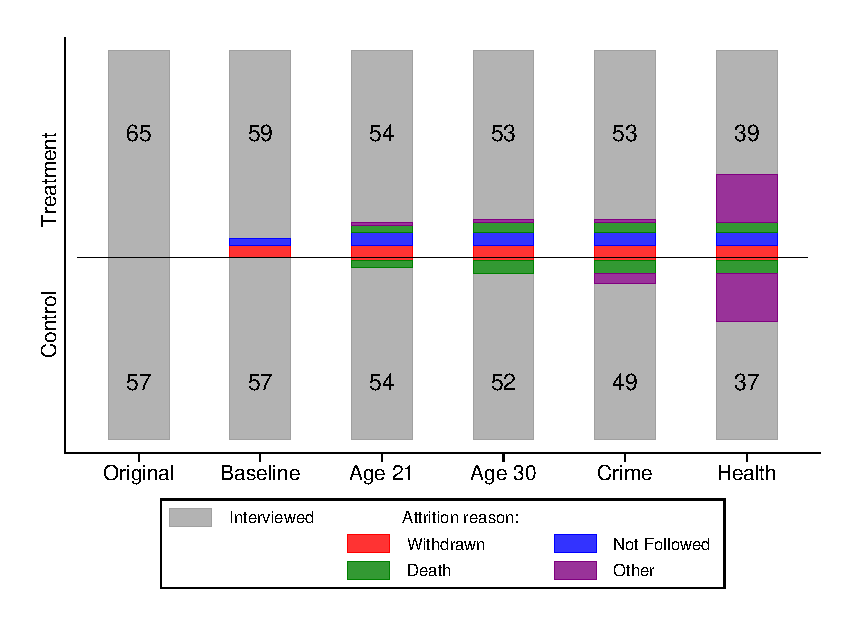
\includegraphics[width=.9\columnwidth]{output/abc_attrition.eps}
  \floatfoot{
\footnotesize
Note: This plot shows the number of participants in ABC for whom there exists data at the periods of data collection by experimental group. The children who withdrew from the study did so due to several reasons, such as adoption. Children were not followed if they were found to be biologically retarded after randomization. The numbers in the bars indicate the number of individuals who were interviewed during that phase of data collection. The original sample was measured after randomization but before the start of the program, the baseline sample was measured at the start of the program, and the health sample was collected at age 34.
}
\end{figure}
\end{comment}

\noindent Attrition was low in ABC. Information is available on 100 subjects in the age 30 follow-up, which we call the adult follow-up. In addition, 80 subjects---40 from the control group and 40 from the treatment group---consented to the release of their criminal records. Further, 70 participants consented to the release of information regarding a full-range biomedical panel---31 from the control group and 39 from the treatment group. \\

\noindent Attrition was also low for CARE subjects. Information is available on 58 subjects (more than 85\% of the initial sample) in the age-30 follow-up. Additionally, 40 participants (11 from the control group, 18 from the family education group, and 11 from the center-based childcare and family education group) released information on the full-range biomedical sweep. Administrative crime data are not available for CARE. We do not evaluate the second-phase of treatment in CARE because it was not randomized.  Rather, those in the center-based childcare and family education group and the family education group were offered school-age treatment, and those in the control group were not. \\

\noindent In the following set of tables (Table~\ref{tab:abc_baseline} through Table~\ref{tab:health_baseline}), we compare the observed, baseline characteristics between the first-phase control and treatment groups in ABC, which are the main groups we analyze, at different stages of the data collection follow-ups. For each observed characteristic, we present the bootstrapped $p$-value associated with the standard $t$-test. We also present the bootstrapped, step-down $p$-value on jointly testing the difference in observed characteristics across the two blocks of variables separated by the horizontal line.\footnote{\citet{Lehmann_Romano_2005_testing}.}\\

\noindent First, we compare the first-phase treatment and control groups on baseline characteristics.

\begin{table}[H]
\captionsetup{singlelinecheck=false,justification=centering}
\caption{First-phase Treatment vs. Control Groups \label{tab:baseline}}

  \begin{threeparttable}
  \begin{tabular}{cccccccc}
  \hline\hline

     &  & \scriptsize{Control} & \scriptsize{Treated} & \scriptsize{Control} & \scriptsize{Treated} & \mc{2}{c}{\scriptsize{$p$-value}} \\  

    \scriptsize{Variable} & \scriptsize{Age} & \scriptsize{Obs.} & \scriptsize{Obs.} & \scriptsize{Mean} & \scriptsize{Mean} & \scriptsize{Single $H_0$} & \scriptsize{Multiple $H_0$} \\ 
    \hline  

    \mc{1}{l}{\scriptsize{Male}} & \mc{1}{c}{\scriptsize{0}} & \mc{1}{c}{\scriptsize{57}} & \mc{1}{c}{\scriptsize{59}} & \mc{1}{c}{\scriptsize{0.438}} & \mc{1}{c}{\scriptsize{0.489}} & \mc{1}{c}{\scriptsize{(0.580)}} & \mc{1}{c}{\scriptsize{(0.700)}} \\  

    \mc{1}{l}{\scriptsize{Birth Weight}} & \mc{1}{c}{\scriptsize{0}} & \mc{1}{c}{\scriptsize{56}} & \mc{1}{c}{\scriptsize{58}} & \mc{1}{c}{\scriptsize{7.191}} & \mc{1}{c}{\scriptsize{6.829}} & \mc{1}{c}{\scriptsize{(0.130)}} & \mc{1}{c}{\scriptsize{(0.205)}} \\  

    \mc{1}{l}{\scriptsize{No. Siblings in Household}} & \mc{1}{c}{\scriptsize{0}} & \mc{1}{c}{\scriptsize{57}} & \mc{1}{c}{\scriptsize{59}} & \mc{1}{c}{\scriptsize{0.750}} & \mc{1}{c}{\scriptsize{0.516}} & \mc{1}{c}{\scriptsize{(0.245)}} & \mc{1}{c}{\scriptsize{(0.425)}} \\  

    \mc{1}{l}{\scriptsize{Birth Year}} & \mc{1}{c}{\scriptsize{0}} & \mc{1}{c}{\scriptsize{57}} & \mc{1}{c}{\scriptsize{59}} & \mc{1}{c}{\scriptsize{1974}} & \mc{1}{c}{\scriptsize{1974}} & \mc{1}{c}{\scriptsize{(0.785)}} & \mc{1}{c}{\scriptsize{(0.865)}} \\ 
    \hline  

    \mc{1}{l}{\scriptsize{Mother's Education}} & \mc{1}{c}{\scriptsize{0}} & \mc{1}{c}{\scriptsize{57}} & \mc{1}{c}{\scriptsize{59}} & \mc{1}{c}{\scriptsize{9.864}} & \mc{1}{c}{\scriptsize{10.505}} & \mc{1}{c}{\scriptsize{\textbf{(0.050)}}} & \mc{1}{c}{\scriptsize{\textbf{(0.090)}}} \\  

    \mc{1}{l}{\scriptsize{Mother's Age}} & \mc{1}{c}{\scriptsize{0}} & \mc{1}{c}{\scriptsize{57}} & \mc{1}{c}{\scriptsize{59}} & \mc{1}{c}{\scriptsize{20.103}} & \mc{1}{c}{\scriptsize{19.564}} & \mc{1}{c}{\scriptsize{(0.555)}} & \mc{1}{c}{\scriptsize{(0.665)}} \\  

    \mc{1}{l}{\scriptsize{Parental Income}} & \mc{1}{c}{\scriptsize{0}} & \mc{1}{c}{\scriptsize{57}} & \mc{1}{c}{\scriptsize{58}} & \mc{1}{c}{\scriptsize{6,211}} & \mc{1}{c}{\scriptsize{7,019}} & \mc{1}{c}{\scriptsize{(0.645)}} & \mc{1}{c}{\scriptsize{(0.720)}} \\  

    \mc{1}{l}{\scriptsize{Mother's IQ}} & \mc{1}{c}{\scriptsize{0}} & \mc{1}{c}{\scriptsize{57}} & \mc{1}{c}{\scriptsize{59}} & \mc{1}{c}{\scriptsize{83.419}} & \mc{1}{c}{\scriptsize{85.393}} & \mc{1}{c}{\scriptsize{(0.360)}} & \mc{1}{c}{\scriptsize{(0.510)}} \\  

    \mc{1}{l}{\scriptsize{Father at Home}} & \mc{1}{c}{\scriptsize{0}} & \mc{1}{c}{\scriptsize{57}} & \mc{1}{c}{\scriptsize{59}} & \mc{1}{c}{\scriptsize{0.346}} & \mc{1}{c}{\scriptsize{0.223}} & \mc{1}{c}{\scriptsize{(0.135)}} & \mc{1}{c}{\scriptsize{(0.270)}} \\  

  \hline\hline
  \end{tabular}
    \begin{tablenotes}
    \scriptsize
    \item 
    Note: This table shows the balance in observed characteristics between the treatment and control groups at baseline.
    For each characteristic, we present the $p$-value from a single hypothesis test.
    We also present the $p$-values from multiple testing, where we collectively test the
    baseline characteristics within the blocks separated by the horizontal line.
    Both $p$-values are two-sided and non-parametric. We construct them 
    based on 1,000 re-draws of the full sample. The estimates we display are the means of 
    the empirical bootstrap distribution. 
    
    \end{tablenotes}
  \end{threeparttable}

\end{table}

\noindent Second, we compare the second-phase treatment and control groups on baseline characteristics.

\begin{table}[H]
\captionsetup{singlelinecheck=false,justification=centering}
\caption{Second-phase Treatment vs. Control Groups \label{tab:baseline_sa}}

  \begin{threeparttable}
  \begin{tabular}{cccccccc}
  \hline\hline

     &  & \scriptsize{Control} & \scriptsize{Treatment} & \scriptsize{Control} & \scriptsize{Treated} & \mc{2}{c}{\scriptsize{$p$-value}} \\  

    \scriptsize{Variable} & \scriptsize{Age} & \scriptsize{Obs.} & \scriptsize{Obs.} & \scriptsize{Mean} & \scriptsize{Mean} & \scriptsize{Single $H_0$} & \scriptsize{Multiple $H_0$} \\ 
    \hline  

    \mc{1}{l}{\scriptsize{Male}} & \mc{1}{c}{\scriptsize{0}} & \mc{1}{c}{\scriptsize{47}} & \mc{1}{c}{\scriptsize{48}} & \mc{1}{c}{\scriptsize{0.551}} & \mc{1}{c}{\scriptsize{0.460}} & \mc{1}{c}{\scriptsize{(0.420)}} & \mc{1}{c}{\scriptsize{(0.552)}} \\  

    \mc{1}{l}{\scriptsize{Birth Weight}} & \mc{1}{c}{\scriptsize{0}} & \mc{1}{c}{\scriptsize{47}} & \mc{1}{c}{\scriptsize{48}} & \mc{1}{c}{\scriptsize{7.084}} & \mc{1}{c}{\scriptsize{6.929}} & \mc{1}{c}{\scriptsize{(0.610)}} & \mc{1}{c}{\scriptsize{(0.700)}} \\  

    \mc{1}{l}{\scriptsize{No. Siblings in Household}} & \mc{1}{c}{\scriptsize{0}} & \mc{1}{c}{\scriptsize{47}} & \mc{1}{c}{\scriptsize{48}} & \mc{1}{c}{\scriptsize{0.748}} & \mc{1}{c}{\scriptsize{0.504}} & \mc{1}{c}{\scriptsize{(0.285)}} & \mc{1}{c}{\scriptsize{(0.445)}} \\  

    \mc{1}{l}{\scriptsize{Birth Year}} & \mc{1}{c}{\scriptsize{0}} & \mc{1}{c}{\scriptsize{47}} & \mc{1}{c}{\scriptsize{48}} & \mc{1}{c}{\scriptsize{1974}} & \mc{1}{c}{\scriptsize{1974}} & \mc{1}{c}{\scriptsize{(0.835)}} & \mc{1}{c}{\scriptsize{(0.915)}} \\ 
    \hline  

    \mc{1}{l}{\scriptsize{Mother's Education}} & \mc{1}{c}{\scriptsize{0}} & \mc{1}{c}{\scriptsize{47}} & \mc{1}{c}{\scriptsize{48}} & \mc{1}{c}{\scriptsize{10.150}} & \mc{1}{c}{\scriptsize{10.388}} & \mc{1}{c}{\scriptsize{(0.480)}} & \mc{1}{c}{\scriptsize{(0.685)}} \\  

    \mc{1}{l}{\scriptsize{Mother's Age}} & \mc{1}{c}{\scriptsize{0}} & \mc{1}{c}{\scriptsize{47}} & \mc{1}{c}{\scriptsize{48}} & \mc{1}{c}{\scriptsize{21.122}} & \mc{1}{c}{\scriptsize{18.884}} & \mc{1}{c}{\scriptsize{\textbf{(0.035)}}} & \mc{1}{c}{\scriptsize{\textbf{(0.065)}}} \\  

    \mc{1}{l}{\scriptsize{Parental Income}} & \mc{1}{c}{\scriptsize{0}} & \mc{1}{c}{\scriptsize{47}} & \mc{1}{c}{\scriptsize{48}} & \mc{1}{c}{\scriptsize{7,589}} & \mc{1}{c}{\scriptsize{6,714}} & \mc{1}{c}{\scriptsize{(0.625)}} & \mc{1}{c}{\scriptsize{(0.795)}} \\  

    \mc{1}{l}{\scriptsize{Mother's IQ}} & \mc{1}{c}{\scriptsize{0}} & \mc{1}{c}{\scriptsize{47}} & \mc{1}{c}{\scriptsize{48}} & \mc{1}{c}{\scriptsize{83.000}} & \mc{1}{c}{\scriptsize{85.831}} & \mc{1}{c}{\scriptsize{(0.185)}} & \mc{1}{c}{\scriptsize{(0.350)}} \\  

    \mc{1}{l}{\scriptsize{Father at Home}} & \mc{1}{c}{\scriptsize{0}} & \mc{1}{c}{\scriptsize{47}} & \mc{1}{c}{\scriptsize{48}} & \mc{1}{c}{\scriptsize{0.279}} & \mc{1}{c}{\scriptsize{0.287}} & \mc{1}{c}{\scriptsize{(0.920)}} & \mc{1}{c}{\scriptsize{(0.965)}} \\  

  \hline\hline
  \end{tabular}
    \begin{tablenotes}
    \scriptsize
    \item 
    Note: This table shows the balance in observed characteristics between the school-age treatment and control groups at baseline.
    For each characteristic, we present the $p$-value from a single hypothesis test.
    We also present the $p$-values from multiple testing, where we collectively test the
    baseline characteristics within the blocks separated by the horizontal line.
    Both $p$-values are two-sided and non-parametric. We construct them 
    based on 200 re-draws of the full sample. The estimates we display are the means of 
    the empirical bootstrap distribution. 
    
    \end{tablenotes}
  \end{threeparttable}

\end{table}

\noindent Third, we compare the observed, baseline characteristics of attrited and non-attrited subjects in the first-phase treatment assignment.

\begin{table}[H]
\captionsetup{singlelinecheck=false,justification=centering}
\caption{Observed vs. Attritted Children, ABC \label{tab:attrition_baseline}}

  \begin{threeparttable}
  \begin{tabular}{cccccccc}
  \toprule

     &  &  &  & \scriptsize{Observed} & \scriptsize{Attritted} & \mc{2}{c}{\scriptsize{$p$-value}} \\  

    \scriptsize{Variable} & \scriptsize{Age} & \scriptsize{Obs.} & \scriptsize{Att.} & \scriptsize{Mean} & \scriptsize{Mean} & \scriptsize{Single $H_0$} & \scriptsize{Multiple $H_0$} \\ 
    \midrule

    \mc{1}{l}{\scriptsize{Male}} & \mc{1}{c}{\scriptsize{0}} & \mc{1}{c}{\scriptsize{103}} & \mc{1}{c}{\scriptsize{13}} & \mc{1}{c}{\scriptsize{0.488}} & \mc{1}{c}{\scriptsize{0.248}} & \mc{1}{c}{\scriptsize{\textbf{(0.085)}}} & \mc{1}{c}{\scriptsize{(0.140)}} \\  

    \mc{1}{l}{\scriptsize{Birth Weight}} & \mc{1}{c}{\scriptsize{0}} & \mc{1}{c}{\scriptsize{103}} & \mc{1}{c}{\scriptsize{11}} & \mc{1}{c}{\scriptsize{7.014}} & \mc{1}{c}{\scriptsize{6.948}} & \mc{1}{c}{\scriptsize{(0.825)}} & \mc{1}{c}{\scriptsize{(0.875)}} \\  

    \mc{1}{l}{\scriptsize{No. Siblings in Household}} & \mc{1}{c}{\scriptsize{0}} & \mc{1}{c}{\scriptsize{103}} & \mc{1}{c}{\scriptsize{13}} & \mc{1}{c}{\scriptsize{0.609}} & \mc{1}{c}{\scriptsize{0.829}} & \mc{1}{c}{\scriptsize{(0.600)}} & \mc{1}{c}{\scriptsize{(0.705)}} \\  

    \mc{1}{l}{\scriptsize{Birth Year}} & \mc{1}{c}{\scriptsize{0}} & \mc{1}{c}{\scriptsize{103}} & \mc{1}{c}{\scriptsize{13}} & \mc{1}{c}{\scriptsize{1974}} & \mc{1}{c}{\scriptsize{1973}} & \mc{1}{c}{\scriptsize{\textbf{(0.045)}}} & \mc{1}{c}{\scriptsize{\textbf{(0.095)}}} \\ 
    \midrule

    \mc{1}{l}{\scriptsize{Mother's Education}} & \mc{1}{c}{\scriptsize{0}} & \mc{1}{c}{\scriptsize{103}} & \mc{1}{c}{\scriptsize{13}} & \mc{1}{c}{\scriptsize{10.302}} & \mc{1}{c}{\scriptsize{9.192}} & \mc{1}{c}{\scriptsize{\textbf{(0.100)}}} & \mc{1}{c}{\scriptsize{(0.165)}} \\  

    \mc{1}{l}{\scriptsize{Mother's Age}} & \mc{1}{c}{\scriptsize{0}} & \mc{1}{c}{\scriptsize{103}} & \mc{1}{c}{\scriptsize{13}} & \mc{1}{c}{\scriptsize{20.016}} & \mc{1}{c}{\scriptsize{18.178}} & \mc{1}{c}{\scriptsize{\textbf{(0.080)}}} & \mc{1}{c}{\scriptsize{(0.160)}} \\  

    \mc{1}{l}{\scriptsize{Mother Employed}} & \mc{1}{c}{\scriptsize{0}} & \mc{1}{c}{\scriptsize{103}} & \mc{1}{c}{\scriptsize{13}} & \mc{1}{c}{\scriptsize{0.268}} & \mc{1}{c}{\scriptsize{0.255}} & \mc{1}{c}{\scriptsize{(0.925)}} & \mc{1}{c}{\scriptsize{(0.955)}} \\  

    \mc{1}{l}{\scriptsize{Parental Income}} & \mc{1}{c}{\scriptsize{0}} & \mc{1}{c}{\scriptsize{103}} & \mc{1}{c}{\scriptsize{12}} & \mc{1}{c}{\scriptsize{6,622}} & \mc{1}{c}{\scriptsize{6,442}} & \mc{1}{c}{\scriptsize{(0.950)}} & \mc{1}{c}{\scriptsize{(0.960)}} \\  

    \mc{1}{l}{\scriptsize{Mother's IQ}} & \mc{1}{c}{\scriptsize{0}} & \mc{1}{c}{\scriptsize{103}} & \mc{1}{c}{\scriptsize{13}} & \mc{1}{c}{\scriptsize{85.050}} & \mc{1}{c}{\scriptsize{78.834}} & \mc{1}{c}{\scriptsize{\textbf{(0.070)}}} & \mc{1}{c}{\scriptsize{(0.135)}} \\  

    \mc{1}{l}{\scriptsize{Father at Home}} & \mc{1}{c}{\scriptsize{0}} & \mc{1}{c}{\scriptsize{103}} & \mc{1}{c}{\scriptsize{13}} & \mc{1}{c}{\scriptsize{0.278}} & \mc{1}{c}{\scriptsize{0.329}} & \mc{1}{c}{\scriptsize{(0.735)}} & \mc{1}{c}{\scriptsize{(0.835)}} \\  

  \bottomrule
  \end{tabular}
    \begin{tablenotes}
    \scriptsize
    \item 
    Note: This table shows the balance in observed characteristics between ABC subjects who were followed up to at least age 21 and ABC subjects who attrited before age 21.
    For each characteristic, we present the $p$-value from a single hypothesis test.
    We also present the $p$-values from multiple hypothesis testing, where we collectively test the
    baseline characteristics within the blocks separated by the horizontal line.
    Both $p$-values are two-sided and non-parametric. We construct them 
    based on 200 re-draws of the full sample. The estimates we display are the means of 
    the empirical bootstrap distribution. 
    
    \end{tablenotes}
  \end{threeparttable}

\end{table}

\noindent Fourth, we compare the observed, baseline characteristics between the subjects in the treatment and the control groups, excluding those who did not comply to treatment.

\begin{table}[H]
\captionsetup{singlelinecheck=false,justification=centering}
\caption{First-stage Treatment vs. Control Groups, Dropping Attrited Children \label{tab:postattrition_baseline}}

  \begin{threeparttable}
  \begin{tabular}{cccccccc}
  \hline\hline

     &  & \scriptsize{Control} & \scriptsize{Treatment} & \scriptsize{Control} & \scriptsize{Treatment} & \mc{2}{c}{\scriptsize{$p$-value}} \\  

    \scriptsize{Variable} & \scriptsize{Age} & \scriptsize{Obs.} & \scriptsize{Obs.} & \scriptsize{Mean} & \scriptsize{Mean} & \scriptsize{Single $H_0$} & \scriptsize{Multiple $H_0$} \\ 
    \hline  

    \mc{1}{l}{\scriptsize{Male}} & \mc{1}{c}{\scriptsize{0}} & \mc{1}{c}{\scriptsize{51}} & \mc{1}{c}{\scriptsize{52}} & \mc{1}{c}{\scriptsize{0.452}} & \mc{1}{c}{\scriptsize{0.524}} & \mc{1}{c}{\scriptsize{(0.430)}} & \mc{1}{c}{\scriptsize{(0.600)}} \\  

    \mc{1}{l}{\scriptsize{Birth Weight}} & \mc{1}{c}{\scriptsize{0}} & \mc{1}{c}{\scriptsize{51}} & \mc{1}{c}{\scriptsize{52}} & \mc{1}{c}{\scriptsize{7.210}} & \mc{1}{c}{\scriptsize{6.822}} & \mc{1}{c}{\scriptsize{(0.115)}} & \mc{1}{c}{\scriptsize{(0.220)}} \\  

    \mc{1}{l}{\scriptsize{No. Siblings in Household}} & \mc{1}{c}{\scriptsize{0}} & \mc{1}{c}{\scriptsize{51}} & \mc{1}{c}{\scriptsize{52}} & \mc{1}{c}{\scriptsize{0.767}} & \mc{1}{c}{\scriptsize{0.455}} & \mc{1}{c}{\scriptsize{(0.150)}} & \mc{1}{c}{\scriptsize{(0.230)}} \\  

    \mc{1}{l}{\scriptsize{Birth Year}} & \mc{1}{c}{\scriptsize{0}} & \mc{1}{c}{\scriptsize{51}} & \mc{1}{c}{\scriptsize{52}} & \mc{1}{c}{\scriptsize{1974}} & \mc{1}{c}{\scriptsize{1974}} & \mc{1}{c}{\scriptsize{(0.635)}} & \mc{1}{c}{\scriptsize{(0.785)}} \\ 
    \hline  

    \mc{1}{l}{\scriptsize{Mother's Education}} & \mc{1}{c}{\scriptsize{0}} & \mc{1}{c}{\scriptsize{51}} & \mc{1}{c}{\scriptsize{52}} & \mc{1}{c}{\scriptsize{10.000}} & \mc{1}{c}{\scriptsize{10.598}} & \mc{1}{c}{\scriptsize{\textbf{(0.085)}}} & \mc{1}{c}{\scriptsize{(0.160)}} \\  

    \mc{1}{l}{\scriptsize{Mother's Age}} & \mc{1}{c}{\scriptsize{0}} & \mc{1}{c}{\scriptsize{51}} & \mc{1}{c}{\scriptsize{52}} & \mc{1}{c}{\scriptsize{20.412}} & \mc{1}{c}{\scriptsize{19.635}} & \mc{1}{c}{\scriptsize{(0.405)}} & \mc{1}{c}{\scriptsize{(0.580)}} \\  

    \mc{1}{l}{\scriptsize{Parental Income}} & \mc{1}{c}{\scriptsize{0}} & \mc{1}{c}{\scriptsize{51}} & \mc{1}{c}{\scriptsize{52}} & \mc{1}{c}{\scriptsize{6,409}} & \mc{1}{c}{\scriptsize{6,846}} & \mc{1}{c}{\scriptsize{(0.765)}} & \mc{1}{c}{\scriptsize{(0.835)}} \\  

    \mc{1}{l}{\scriptsize{Mother's IQ}} & \mc{1}{c}{\scriptsize{0}} & \mc{1}{c}{\scriptsize{51}} & \mc{1}{c}{\scriptsize{52}} & \mc{1}{c}{\scriptsize{84.472}} & \mc{1}{c}{\scriptsize{85.635}} & \mc{1}{c}{\scriptsize{(0.560)}} & \mc{1}{c}{\scriptsize{(0.715)}} \\  

    \mc{1}{l}{\scriptsize{Father at Home}} & \mc{1}{c}{\scriptsize{0}} & \mc{1}{c}{\scriptsize{51}} & \mc{1}{c}{\scriptsize{52}} & \mc{1}{c}{\scriptsize{0.349}} & \mc{1}{c}{\scriptsize{0.208}} & \mc{1}{c}{\scriptsize{(0.115)}} & \mc{1}{c}{\scriptsize{(0.225)}} \\  

  \hline\hline
  \end{tabular}
    \begin{tablenotes}
    \scriptsize
    \item 
    Note: This table shows the balance in observed characteristics between the treatment and control groups of subjects who were followed up to at least age 21.
    For each characteristic, we present the $p$-value from a single hypothesis test.
    We also present the $p$-values from multiple testing, where we collectively test the
    baseline characteristics within the blocks separated by the horizontal line.
    Both $p$-values are two-sided and non-parametric. We construct them 
    based on 1,000 re-draws of the full sample. The estimates we display are the means of 
    the empirical bootstrap distribution. 
    
    \end{tablenotes}
  \end{threeparttable}

\end{table}

\begin{comment}
\noindent Fifth, we compare the observed baseline characteristics between the subjects in the first-phase treatment, restricting the sample to those who consented to release their age-34 criminal records.

\begin{table}[H]
\captionsetup{singlelinecheck=false,justification=centering}
\caption{First-phase Treatment vs. Control Groups, Subjects who Released Criminal Records  \label{tab:crime_baseline}}

  \begin{threeparttable}
  \begin{tabular}{cccccccc}
  \hline\hline

     &  & \scriptsize{Control} & \scriptsize{Treatment} & \scriptsize{Control} & \scriptsize{Treatment} & \mc{2}{c}{\scriptsize{$p$-value}} \\  

    \scriptsize{Variable} & \scriptsize{Age} & \scriptsize{Obs.} & \scriptsize{Obs.} & \scriptsize{Mean} & \scriptsize{Mean} & \scriptsize{Single $H_0$} & \scriptsize{Multiple $H_0$} \\ 
    \hline  

    \mc{1}{l}{\scriptsize{Male}} & \mc{1}{c}{\scriptsize{0}} & \mc{1}{c}{\scriptsize{45}} & \mc{1}{c}{\scriptsize{43}} & \mc{1}{c}{\scriptsize{0.423}} & \mc{1}{c}{\scriptsize{0.527}} & \mc{1}{c}{\scriptsize{(0.275)}} & \mc{1}{c}{\scriptsize{(0.425)}} \\  

    \mc{1}{l}{\scriptsize{Birth Weight}} & \mc{1}{c}{\scriptsize{0}} & \mc{1}{c}{\scriptsize{45}} & \mc{1}{c}{\scriptsize{43}} & \mc{1}{c}{\scriptsize{7.226}} & \mc{1}{c}{\scriptsize{6.940}} & \mc{1}{c}{\scriptsize{(0.295)}} & \mc{1}{c}{\scriptsize{(0.415)}} \\  

    \mc{1}{l}{\scriptsize{No. Siblings in Household}} & \mc{1}{c}{\scriptsize{0}} & \mc{1}{c}{\scriptsize{45}} & \mc{1}{c}{\scriptsize{43}} & \mc{1}{c}{\scriptsize{0.780}} & \mc{1}{c}{\scriptsize{0.491}} & \mc{1}{c}{\scriptsize{(0.220)}} & \mc{1}{c}{\scriptsize{(0.340)}} \\  

    \mc{1}{l}{\scriptsize{Birth Year}} & \mc{1}{c}{\scriptsize{0}} & \mc{1}{c}{\scriptsize{45}} & \mc{1}{c}{\scriptsize{43}} & \mc{1}{c}{\scriptsize{1975}} & \mc{1}{c}{\scriptsize{1974}} & \mc{1}{c}{\scriptsize{(0.520)}} & \mc{1}{c}{\scriptsize{(0.680)}} \\ 
    \hline  

    \mc{1}{l}{\scriptsize{Mother's Education}} & \mc{1}{c}{\scriptsize{0}} & \mc{1}{c}{\scriptsize{45}} & \mc{1}{c}{\scriptsize{43}} & \mc{1}{c}{\scriptsize{9.947}} & \mc{1}{c}{\scriptsize{10.485}} & \mc{1}{c}{\scriptsize{(0.125)}} & \mc{1}{c}{\scriptsize{(0.210)}} \\  

    \mc{1}{l}{\scriptsize{Mother's Age}} & \mc{1}{c}{\scriptsize{0}} & \mc{1}{c}{\scriptsize{45}} & \mc{1}{c}{\scriptsize{43}} & \mc{1}{c}{\scriptsize{20.273}} & \mc{1}{c}{\scriptsize{19.571}} & \mc{1}{c}{\scriptsize{(0.530)}} & \mc{1}{c}{\scriptsize{(0.660)}} \\  

    \mc{1}{l}{\scriptsize{Parental Income}} & \mc{1}{c}{\scriptsize{0}} & \mc{1}{c}{\scriptsize{45}} & \mc{1}{c}{\scriptsize{43}} & \mc{1}{c}{\scriptsize{5,751}} & \mc{1}{c}{\scriptsize{7,437}} & \mc{1}{c}{\scriptsize{(0.355)}} & \mc{1}{c}{\scriptsize{(0.495)}} \\  

    \mc{1}{l}{\scriptsize{Mother's IQ}} & \mc{1}{c}{\scriptsize{0}} & \mc{1}{c}{\scriptsize{45}} & \mc{1}{c}{\scriptsize{43}} & \mc{1}{c}{\scriptsize{84.612}} & \mc{1}{c}{\scriptsize{85.504}} & \mc{1}{c}{\scriptsize{(0.655)}} & \mc{1}{c}{\scriptsize{(0.785)}} \\  

    \mc{1}{l}{\scriptsize{Father at Home}} & \mc{1}{c}{\scriptsize{0}} & \mc{1}{c}{\scriptsize{45}} & \mc{1}{c}{\scriptsize{43}} & \mc{1}{c}{\scriptsize{0.334}} & \mc{1}{c}{\scriptsize{0.256}} & \mc{1}{c}{\scriptsize{(0.390)}} & \mc{1}{c}{\scriptsize{(0.550)}} \\  

  \hline\hline
  \end{tabular}
    \begin{tablenotes}
    \scriptsize
    \item 
    Note: This table shows the balance in observed characteristics between the treatment and control groups at baseline for subjects who consented to release their administrative criminal records.
    For each characteristic, we present the $p$-value from a single hypothesis test.
    We also present the $p$-values from multiple testing, where we collectively test the
    baseline characteristics within the blocks separated by the horizontal line.
    Both $p$-values are two-sided and non-parametric. We construct them 
    based on 1,000 re-draws of the full sample. The estimates we display are the means of 
    the empirical bootstrap distribution. 
    
    \end{tablenotes}
  \end{threeparttable}

\end{table}
\end{comment}

\noindent Finally, we compare the observed, baseline characteristics between the children in the first-phase treatment, restricting the sample to the children for whom we have information on the age-34 medical data collection. \textbf{[JJH: Why carrow so many age ``0'' levels?] [JLG: I worry that the referees are skeptical about the pureness of the randomization protocol and that's why we are including as many evidence as possible on baseline balance. If you prefer we can place in a holding tank.]}

\begin{table}[H]
\captionsetup{singlelinecheck=false,justification=centering}
\caption{First-phase Treatment vs. Control Groups, Children who Completed the Medical Sweep Follow-up, ABC \label{tab:health_baseline}}

  \begin{threeparttable}
  \begin{tabular}{cccccccc}
  \hline\hline

     &  & \scriptsize{Control} & \scriptsize{Treated} & \scriptsize{Control} & \scriptsize{Treated} & \mc{2}{c}{\scriptsize{$p$-value}} \\  

    \scriptsize{Variable} & \scriptsize{Age} & \scriptsize{Obs.} & \scriptsize{Obs.} & \scriptsize{Mean} & \scriptsize{Mean} & \scriptsize{Single $H_0$} & \scriptsize{Multiple $H_0$} \\ 
    \hline  

    \mc{1}{l}{\scriptsize{Male}} & \mc{1}{c}{\scriptsize{0}} & \mc{1}{c}{\scriptsize{31}} & \mc{1}{c}{\scriptsize{39}} & \mc{1}{c}{\scriptsize{0.293}} & \mc{1}{c}{\scriptsize{0.533}} & \mc{1}{c}{\scriptsize{\textbf{(0.050)}}} & \mc{1}{c}{\scriptsize{\textbf{(0.055)}}} \\  

    \mc{1}{l}{\scriptsize{Birth Weight}} & \mc{1}{c}{\scriptsize{0}} & \mc{1}{c}{\scriptsize{31}} & \mc{1}{c}{\scriptsize{39}} & \mc{1}{c}{\scriptsize{7.233}} & \mc{1}{c}{\scriptsize{6.826}} & \mc{1}{c}{\scriptsize{(0.190)}} & \mc{1}{c}{\scriptsize{(0.295)}} \\  

    \mc{1}{l}{\scriptsize{No. Siblings in Household}} & \mc{1}{c}{\scriptsize{0}} & \mc{1}{c}{\scriptsize{31}} & \mc{1}{c}{\scriptsize{39}} & \mc{1}{c}{\scriptsize{0.613}} & \mc{1}{c}{\scriptsize{0.493}} & \mc{1}{c}{\scriptsize{(0.580)}} & \mc{1}{c}{\scriptsize{(0.750)}} \\  

    \mc{1}{l}{\scriptsize{Birth Year}} & \mc{1}{c}{\scriptsize{0}} & \mc{1}{c}{\scriptsize{31}} & \mc{1}{c}{\scriptsize{39}} & \mc{1}{c}{\scriptsize{1975}} & \mc{1}{c}{\scriptsize{1974}} & \mc{1}{c}{\scriptsize{(0.360)}} & \mc{1}{c}{\scriptsize{(0.510)}} \\ 
    \hline  

    \mc{1}{l}{\scriptsize{Mother's Education}} & \mc{1}{c}{\scriptsize{0}} & \mc{1}{c}{\scriptsize{31}} & \mc{1}{c}{\scriptsize{39}} & \mc{1}{c}{\scriptsize{10.039}} & \mc{1}{c}{\scriptsize{10.597}} & \mc{1}{c}{\scriptsize{(0.190)}} & \mc{1}{c}{\scriptsize{(0.385)}} \\  

    \mc{1}{l}{\scriptsize{Mother's Age}} & \mc{1}{c}{\scriptsize{0}} & \mc{1}{c}{\scriptsize{31}} & \mc{1}{c}{\scriptsize{39}} & \mc{1}{c}{\scriptsize{19.389}} & \mc{1}{c}{\scriptsize{19.595}} & \mc{1}{c}{\scriptsize{(0.825)}} & \mc{1}{c}{\scriptsize{(0.945)}} \\  

    \mc{1}{l}{\scriptsize{Mother Employed}} & \mc{1}{c}{\scriptsize{0}} & \mc{1}{c}{\scriptsize{31}} & \mc{1}{c}{\scriptsize{39}} & \mc{1}{c}{\scriptsize{0.195}} & \mc{1}{c}{\scriptsize{0.349}} & \mc{1}{c}{\scriptsize{(0.185)}} & \mc{1}{c}{\scriptsize{(0.315)}} \\  

    \mc{1}{l}{\scriptsize{Parental Income}} & \mc{1}{c}{\scriptsize{0}} & \mc{1}{c}{\scriptsize{31}} & \mc{1}{c}{\scriptsize{39}} & \mc{1}{c}{\scriptsize{5,509}} & \mc{1}{c}{\scriptsize{7,520}} & \mc{1}{c}{\scriptsize{(0.280)}} & \mc{1}{c}{\scriptsize{(0.535)}} \\  

    \mc{1}{l}{\scriptsize{Mother's IQ}} & \mc{1}{c}{\scriptsize{0}} & \mc{1}{c}{\scriptsize{31}} & \mc{1}{c}{\scriptsize{39}} & \mc{1}{c}{\scriptsize{83.822}} & \mc{1}{c}{\scriptsize{84.922}} & \mc{1}{c}{\scriptsize{(0.655)}} & \mc{1}{c}{\scriptsize{(0.860)}} \\  

    \mc{1}{l}{\scriptsize{Father at Home}} & \mc{1}{c}{\scriptsize{0}} & \mc{1}{c}{\scriptsize{31}} & \mc{1}{c}{\scriptsize{39}} & \mc{1}{c}{\scriptsize{0.355}} & \mc{1}{c}{\scriptsize{0.231}} & \mc{1}{c}{\scriptsize{(0.205)}} & \mc{1}{c}{\scriptsize{(0.450)}} \\  

  \hline\hline
  \end{tabular}
    \begin{tablenotes}
    \scriptsize
    \item 
    Note: This table shows the balance in observed characteristics between the treatment and control groups in ABC at baseline for subjects who completed the health follow-up at age 34.
    For each characteristic, we present the $p$-value from a single hypothesis test.
    We also present the $p$-values from multiple testing, where we collectively test the
    baseline characteristics within the blocks separated by the horizontal line.
    Both $p$-values are two-sided and non-parametric. We construct them 
    based on 200 re-draws of the full sample. The estimates we display are the means of 
    the empirical bootstrap distribution. 
    
    \end{tablenotes}
  \end{threeparttable}

\end{table}

\noindent Despite some exceptions, these tables indicate balance between the treatment and control groups from the first-phase randomization, which is the primary comparison we analyze in the main paper. The balance in observed characteristics holds for the different samples we consider, which differs from the initial sample due to various instances of item non-response. For the second-phase randomization, there is also balance in observed characteristics. \\

\subsubsection{Summary of Data Collection} \label{appendix:data-collection}

Data across a wide range of outcomes were collected for ABC and CARE at similar time points. Table~\ref{tab:abc-care-data} summarizes the data collection for both programs. A varied battery of measures of cognitive, social-emotional, and parenting skills were administered during the intervention and while the children were in school. Adult follow-ups are available at ages 21, 30, and 34, with administrative crime records and biomarker health data available at age 34.

\begin{table}[H]
\centering
\caption{ABC and CARE Data Collection}
\label{tab:abc-care-data}
\begin{threeparttable}
\footnotesize
	\begin{tabular}{l l l l}
\toprule
Variable & Early & School-age & Adult  \\
\midrule
\textbf{Family} & 0, 1.5, 2.5, 3.5, 4.5 & 8 & \\
\textbf{Cognitive} & \\
\quad IQ & 2, 2.5, 3, 3.5, 4, 4.5, 5 & 6*, 6.5, 7, 8, 12, 15* & 21* \\
\quad Achievement &  & 5.5, 6, 6.5, 7, 7.5, 8, 8.5, 9, 12, 15 * & 21\\
\textbf{Social-emotional} & & & \\
\quad Task orientation & 3 m.*, 6 m., 9 m.*, 1, 1.5, 2  & 5.5, 6, 6.5, 7.5& \\
\quad Extraversion & & 5.5, 6, 6.5, 7, 7.5, 8, 12 & \\
\quad Behavior &  & 8, 12, 15* & \\ 
\textbf{Parenting} & 6 m., 1.5, 2.5, 3.5*, 4.5* & 8* & \\
\textbf{Education} & & 12, 15 & 21, 30 \\
\textbf{Labor} & & & 21, 30 \\
\textbf{Parental income} & 0, 1.5, 2.5, 3.5, 4.5 & 8 & 21 \\
\textbf{Health} & 0, 1.5, 2.5, 3.5, 4.5 & 8 & 21, 30, 34 \\
\textbf{Crime} & & & 21, 30, 34 \\
\bottomrule
\end{tabular}
\begin{tablenotes}
\footnotesize
\item Note: This table provides an abbreviated summary of the variables available in ABC and CARE. The cognitive and social-emotional categories listed are a subset of the full list of measured skills. Ages followed by m.\ are in months. All other ages are in years. Ages with an asterisk (*) are only present in ABC.
\end{tablenotes}
\end{threeparttable}
\end{table}
